\documentclass[a4paper,titlepage,openright,12pt]{report}
\usepackage{graphicx}
%\usepackage{epsfig}
\usepackage[font=footnotesize]{subfig}
\usepackage{float}
\usepackage{fancyhdr}
\usepackage{makeidx}
\usepackage[nottoc,notlot,notlof]{tocbibind}
\usepackage{supertabular}
\usepackage{array}
\usepackage{setspace}
\usepackage{enumerate}
\usepackage{rotating}
\usepackage{moreverb}
\usepackage{multirow}
\usepackage{amsmath}
\usepackage{amsthm}
\usepackage{amssymb}
\usepackage{captcont}
\usepackage{verbatim}
\usepackage{titlesec}
\usepackage{url}
\usepackage{hyperref}
\usepackage{lipsum}
\usepackage{tabularx}
\usepackage{url}
\usepackage[algoruled]{algorithm2e}
%\usepackage[figure,algoruled]{algorithm2e}
%\usepackage[figure,boxruled]{algorithm2e}

%\newtheorem{theorem}{Theorem}
%\newtheorem{corollary}[theorem]{Corollary}
%\newtheorem{conjecture}[theorem]{Conjecture}
%\newtheorem{lemma}[theorem]{Lemma}
%\newtheorem{proposition}[theorem]{Proposition}
%\newtheorem{definition}[theorem]{Definition}
%\newtheorem{Example}[theorem]{Example}
%\newtheorem{axiom}{Axiom}
%\newtheorem{remark}{Remark}
%\newtheorem{exercise}{Exercise}[section]
%\newtheorem{fact}[theorem]{Fact}
%\newtheorem{property}[theorem]{Property}
\setlength{\parindent}{0pt}%for paragraph spacing
\setlength{\parskip}{1ex plus 0.5ex minus 0.2ex}
\setlength{\textheight}{8.5in}
\pagestyle{fancy}
% with this we ensure that the chapter and section
% headings are in lowercase.
%\renewcommand{\bibname}{References}
\renewcommand{\chaptermark}[1]{\markboth{#1}{}}
\renewcommand{\sectionmark}[1]{\markright{\thesection\ #1}}
\fancyhf{} % delete current setting for header and footer
\fancyhead[LE,RO]{\bfseries\thepage}
\fancyhead[LO]{\bfseries\rightmark}
\fancyhead[RE]{\bfseries\leftmark}
%\rfoot{\bfseries\thepage}
\cfoot{\em $\copyright$ 2015-16, Indian Institute of Technology Delhi}
\renewcommand{\headrulewidth}{0.5pt}
\renewcommand{\footrulewidth}{0.5pt}
\addtolength{\headheight}{2.5pt} % make space for the rule

\fancypagestyle{plain}{%
\fancyhead{} % get rid of headers on plain pages
\fancyfoot{}
%\rfoot{\bfseries\thepage}
\cfoot{\em $\copyright$ 2015-16, Indian Institute of Technology Delhi}
\renewcommand{\headrulewidth}{0pt} % and the line
}

%% The smart version of cleardouble page.
\let\origdoublepage\cleardoublepage
\newcommand{\clearemptydoublepage}{%
  \clearpage
  {\pagestyle{empty}\origdoublepage}%
}

\let\cleardoublepage\clearemptydoublepage


\date{}


\addtolength{\oddsidemargin}{30pt}
\addtolength{\evensidemargin}{-40pt}

\titlespacing*{\chapter}{0pt}{-50pt}{20pt}
\titleformat{\chapter}[display]{\normalfont\huge\bfseries}{\chaptertitlename\ \thechapter}{20pt}{\Huge}
% \DeclareGraphicsExtensions{.pdf,.png,.jpg,.ps}
\floatstyle{boxed}
\restylefloat{figure}
\setcounter{lofdepth}{2}
\setcounter{lotdepth}{2}

\newtheorem{claim}{Claim}[section]
\newtheorem{theorem}{Theorem}[section]
\newtheorem{defn}{Definition}[section]
\newtheorem{fact}{Fact}[section]

\graphicspath{{./Figures/}}
\begin{document}

%\begin{comment}
% Begin title page
\begin{titlepage}
\begin{center}

\LARGE{\textsf{\bfseries The Corporate-Political Nexus}}\\
\vspace{20pt}
\normalsize
\emph{A thesis submitted in fulfillment} \\
\emph{of the requirements for} \\
\vspace{20pt}
\bfseries M.TECH MAJOR PROJECT \\
%\vspace{20pt}
%\emph {in}\\
%\vspace{20pt}
%\bfseries Deptartment of Computer Science \& Engineering \\
%\vspace{20pt}
\emph {by}\\
\vspace{20pt}
\Large{\textsf{\bfseries ABHISHEK AGARWAL}} \\
{\normalsize \textsf{\bfseries Entry No. 2014MCS2114}}\\

\ \\
%\ \\
{\normalsize \emph {Under the guidance of}}
\ \\
\Large{\textsf{\bfseries Dr. AADITESHWAR SETH}} \\
\ \\
\vspace{30pt}
%\begin{center}

\includegraphics[scale=0.2]{iit_logo.pdf} \\
\vspace{10pt}
%\end{center}
\large{\textsc{Department of Computer Science and Engineering,\\
Indian Institute of Technology Delhi.\\ June 2016.}}
\end{center}
\end{titlepage}

%\newpage
%\cleardoublepage
\onehalfspacing
\thispagestyle{empty}

\normalfont
\begin{center}
\LARGE{ Certificate}
\end{center}

\vspace{0.5in}

This is to certify that the thesis titled {\bfseries The Corporate-Political Nexus} being submitted by
{\bfseries AMARTYA CHAUDHURI} for the award of {\bfseries Master of Technology} in {\bfseries Computer Science \& Engineering} is a record of bona fide work carried out by him under my guidance and supervision at the {\bfseries Department of Computer Science \& Engineering}. The work presented in this thesis has not been submitted elsewhere either in part or full, for the award of any other degree or diploma.

\vspace{1.5in}


{\bfseries Dr. AADITESHWAR SETH} \\
{\bfseries Department of Computer Science and Engineering} \\
{\bfseries Indian Institute of Technology, Delhi}\\

\thispagestyle{empty}
%\begin{center}
\LARGE{Acknowledgments}  %This is the correct spelling dont change sit
\end{center}

\vspace{0.5in}

%Replace \lipsum with your acknowledgement
%\lipsum[1]
I would like to express my heartiest gratitude to my supervisor Dr. Aaditeshwar Seth for guiding this work with utmost interest and scientific rigor. I thank him for setting high standards, giving me freedom to explore multiple facets of the problem and teaching me the value of analytical thinking and hard work. I am also grateful to Manoj Kumar, Anirban Sen and Dipanjan Chakraborty who have helped a great deal by providing their support during difficult times and whose suggestions went a long way in making this work a reality. I am highly indebted to Preeti Rani, Mridul Goel and Md. Imran for actually sitting with me and working on perfecting the final system. I would also like to thank my family and friends for their love and support and bearing with me for my constant absence.\\

\vspace{1.5in}

{\bfseries ABHISHEK AGARWAL}


\thispagestyle{empty}


% \setcounter{page}{1}
% \pagenumbering{roman}
\thispagestyle{empty}
\begin{center}
\LARGE{Abstract}
\end{center}

\vspace{0.5in}

%replace \lipsum with your abstract
%\lipsum[1]
In this project we try to facilitate the study of distribution of power across and within various Indian power institutions by analysing their inter-linkages, family trees, timelines, transactions, etc. to make more sense of the big political and corporate handshakes. In that direction, we envision to construct a system to collect data in this regard from various sources and integrate all of it into a single data store for others to use.

Our aim is to disseminate these findings to the mass society using a crowdsourced system, and use mass language for such a flow of information. and in this way, enhance governmental accountability and transparency using the notion of Open data and crowdsourcing.



\thispagestyle{empty}
\begin{center}
\LARGE{Acknowledgments}  %This is the correct spelling dont change sit
\end{center}

\vspace{0.5in}

%Replace \lipsum with your acknowledgement
%\lipsum[1]
I would like to express my heartiest gratitude to my supervisor Dr. Aaditeshwar Seth for guiding this work with utmost interest and scientific rigor. I thank him for setting high standards, giving me freedom to explore multiple facets of the problem and teaching me the value of analytical thinking and hard work. I am also grateful to Manoj Kumar, Anirban Sen and Dipanjan Chakraborty who have helped a great deal by providing their support during difficult times and whose suggestions went a long way in making this work a reality. I am highly indebted to Preeti Rani, Mridul Goel and Md. Imran for actually sitting with me and working on perfecting the final system. I would also like to thank my family and friends for their love and support and bearing with me for my constant absence.\\

\vspace{1.5in}

{\bfseries ABHISHEK AGARWAL}



\thispagestyle{empty}
\tableofcontents

\thispagestyle{empty}

\listoffigures

\listoftables
%\end{comment}

\thispagestyle{empty}
\cleardoublepage
\onehalfspacing
%%%%%%%%%%%%%%%%%%%%%%%%%%%%%%%%%%%%%%%%%%%%%%%%%%%%%%%%%%%%

\setcounter{page}{1}
\pagenumbering{arabic}

%You may have as many chapters as you please. This is just for reference.

\chapter{Introduction}

%Replace \lipsum with text.
% You may have as many sections as you please. This is just for reference.

This thesis is a document to record our endeavour to tackle the problem of forming the social networks of Indian Politicians and Corporates and analysing them.

\section{Objective}
%\lipsum[1]

%You should cite papers in the following manner: Bayliss et al.~\cite{Bay1} gave an iterative method for Helmholtz equation etc.
%Similar work has been done in \cite{Bailey,Ernst,Gold3}.
The main idea is to collect data from semantic web (and other sources) to form a database ( here onwards we call it the \textbf{knowledge base} or \textbf{knowledge graph} )  and use it to for monitoring the top players in Indian society - mainly in the spheres of politics and businesses in India. We sought answers to questions like - 
\begin{itemize}
    \item \emph{Who were the big players in Indian politics and businesses?}
    \item \emph{Is there any influence (or possibility of it) of political field by a person in corporate field?}
    \item \emph{How important is one politician in a network of politicians (or a businessperson in a business network)?}
    \item \emph{On whom does actual power reside in a democracy?}
\end{itemize}

\section{Motivation \& Related Work}

In his book \textbf{The Power Elite} \cite{Mills}, C. Wright Mills calls attention to the interwoven interests of the leaders of the military, corporate, and political elements of society and suggests that the ordinary citizen is a relatively powerless subject of manipulation by those entities. His book deals with the power elite in US. But the hierarchy he proposes is more or less the same across all countries. Power rests with the top one percent in an economy. We plan to create a watchdog for that one percent. One interesting list to accompany this direction could be the Forbes list \cite{FORBES} of 147 companies that control everything. 

French economist Thomas Piketty in his famous work \textbf{Capital in the Twenty-First Century} \cite{Piketty} focuses on wealth and income inequality in Europe and the United States since the beginning of the industrial revolution. He proposes a global system of progressive wealth taxes to help reduce inequality and avoid the vast majority of wealth coming under the control of a tiny minority. We plan to collect, integrate, visualize and open such data for Indian terrain to let data fanatics carry out sych works to understand this inequality.

British writer and historian Patrick French, in his book \textbf{India: A Potrait} \cite{French} has stated many such interesting patterns in Indian politics where he argues that almost all of the young Indian politicians in the Indian Parliament are hereditary. Infact, patterns similar to this can be seen over the entire political Indian scene. One can find interesting overlaps, family ties, social links within these power houses. In a survey, \textbf{Who owns your media?} \cite{Media}, we find that even the media is an entity of importance and most of the politicians tend to try pull their strings in this domain. Another interesting case could be Jayant Sinha's family tree \cite{Sinha} and their business holdings. He is the Minister of State for Finance and a Member of Indian Parliament and has links to lot of powerful companies.

Research along the area have been prominent across countries. \textbf{Sastry} \cite{Sastry} shows how crime and money play important role in Indian elections. In a related work \textbf{Vaishnav} \cite{Essay} explain why do Indian parties elect criminal candidates and why they win. \textbf{Kapur} \cite{Builders} connects the hidden relationships between politicians and builders. He argues that where elections are costly but accountability mechanisms are weak, politicians often turn to private firms for illicit election finance and that where firms are highly regulated, politicians can exchange policy discretion or regulatory forbearance for bribes and monetary transfers from firms

Works like what we propose have already been done for countries like USA, UK, Chile etc. We have examples like \textbf{LittleSis} \cite{LilSis}, \textbf{Poderopedia} \cite{PODERO} where journalists, developers, analysts came together to put up profiles of important entities, institutions of the society and highlighted the connections between them. Littlesis (opposite of Big brother) in one hand exists in USA from the political and economical data available there. Poderopedia is a similar site in Chile. These sites feature separate pages of people in power in USA, their connections to different institutions and other entities , work history, visualizations of the connections to educate masses etc. Other than producing awareness to people about the corporate- political connections, these sites also allow public to register and collaborate in data entry processes and has an API system to promote further use of their data for research purposes.

Such system in absence of digital data/ structured data and other human factors is difficult in India. But various local and national initiatives have been started. \textbf{Association for democratic Reforms} \cite{ADR} for example has sites like \textbf{Myneta} \cite{MyNeta} to disseminate information about political leaders of India.	

Our vision is to produce a system similar in lines to the websites embedded with the power to query interesting connections, find interesting visualizations, and help raise suspicious issues.

\section{Merits}

The creation of such a system is beneficial for the society as a whole. It disemminates current information to public (or forms an indirect media for the same) which brings about accountability and transparency in the democracy. The project in the long run, helps to create a neat, structured minimal error data collection which otherwise is scattered at respective sources. Moreover, it also acts as a mashup data from different domains to be further used by journalists and academecians etc. Alongwith this, our work shows how such system of inter-disciplinary helps to find patterns and discover more informationa (with the challenges of building up a wiki based system to circulate information) .

\section{Detailed Goals}
In regard to above ideas, we splitted our goals to following objectives - 
\begin{enumerate}
    \item \textbf{Create a structured knowledgebase of corporate-political data.}
        Our main motive was to collect noisy semi structured data from various sources was the first problem encountered. This was followed by the task of entity resolution to merge repeated information pertaining to a single person. Finally the data was fitted into a model for easy queries.
    \item \textbf{Create a web portal to share and/or spread the information contained in the database.}
        The idea was to visualize the data contained in the knowledgebase. In lines with littlesis, we wanted to create a portal to show the networks obtained through different sources and add a wiki to add more through the crowd. Moreover, we also tried to give a minimal query engine to allow users to make custom queries for further analysis. We also wanted to create read/write apis to our knowledge database to help app writers to easily extend it to their applications.
    \item \textbf{Analysis to find patterns in data.}
        Our endeavour is to use the knowledge graph and the query engine we tried to build to look into the network properties and find new patterns and information out of it.

\end{enumerate}
% You may add figures in the following manner.
%\begin{figure}[here]
%\begin{center}	
%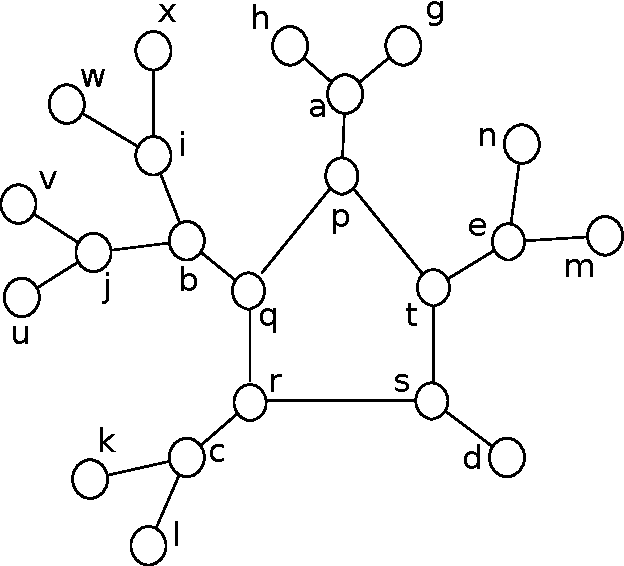
\includegraphics[scale=0.4]{pent} 
%\caption{Pentagon $pqrst$}
%\label{fig:pent}
%\end{center}
%\end{figure}

%\lipsum[1]

%\section{SECTION NAME}
%\lipsum[2]

%\begin{table}
%\centering
%\begin{tabular}{| c | c |}
%\hline
%{\bf item 1} & {\bf item 2} \\ \hline
%
%abcde & 5 \\ \hline
%
%pqrst & 4 \\ \hline
%\end{tabular}
%\caption{A sample table}
%\label{table:1}
%\end{table}


\chapter{System Design}

%Replace \lipsum with text.
% You may have as many sections as you please. This is just for reference.

\section{High Level Design}
%\lipsum[2]
% You may add figures in the following manner.

\begin{figure}[here]
\begin{center}	
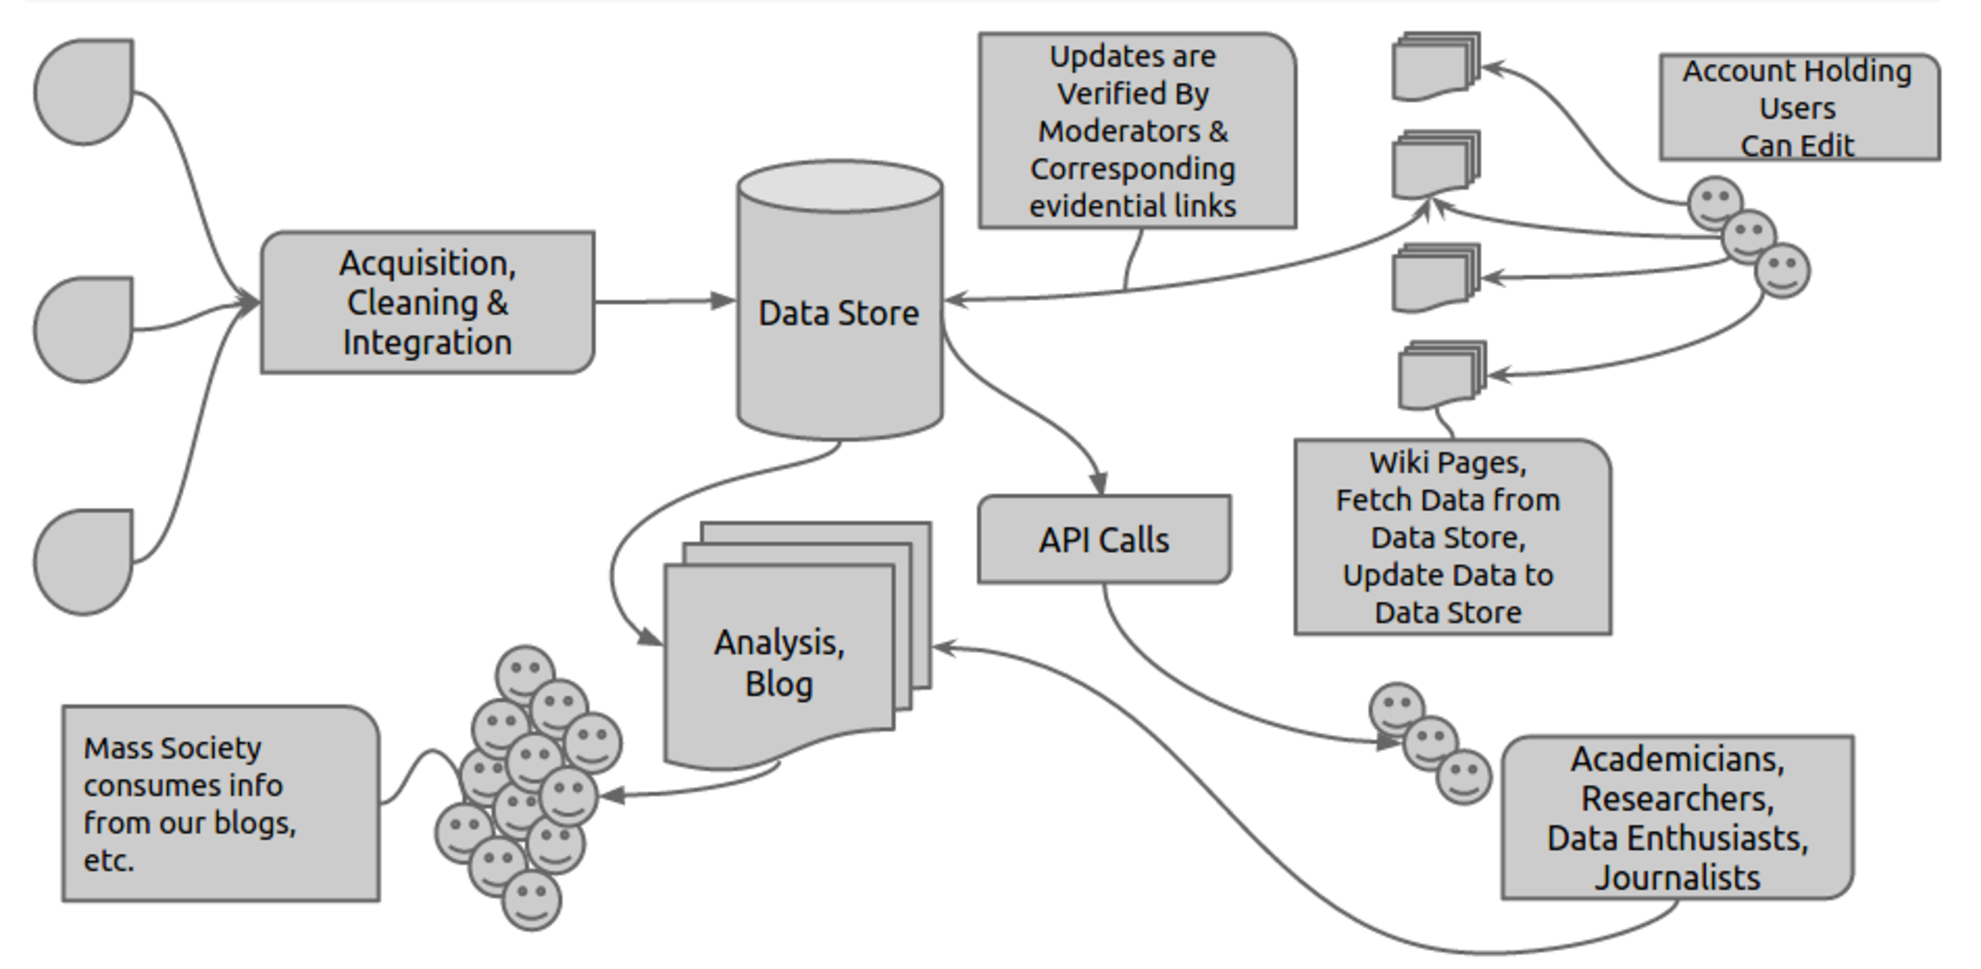
\includegraphics[scale=0.4]{big_pic} 
\caption{Big Picture}
\label{fig:big_pic}
\end{center}
\end{figure}

Above is the generic high level diagram of the entire system as we deduced from our study of the websites above.
We have assumed three main types of users of here:
\begin{enumerate}
\item\textbf{General public} - Use the system for information and news. May also contribute towards data entry.
\item\textbf{Researchers \& Academicians} - Use the site for using social network studies.
\item\textbf{Journalists (Media persons)} - Use the data to frame their news stories.
\end{enumerate}


And keeping these in mind, the system accounts for following functions:
\begin{itemize}
\item\textbf{Data acquisition} - As getting structured data is often difficult system should have a mechanism to automate collection of data from various sources over internet.
\item\textbf{Data Store}  - There should be a central repository for whatever data collected. This repo will store the data in structured form. Care should be taken to keep its integrity, durability and non-redundancy.
\item\textbf{Data Verification} - As the data is sensitive and important, provisions for verification for the input data has to be taken care of. This involves manual labor and system should incorporate this in the entire process.
\item\textbf{Data Visualization} - A portal for the public display of data (in tables, visualizations etc.).
\item\textbf{APIs} - To provide our data for use with other applications.
\end{itemize}

\section{Technical design}
%\lipsum[3]
Accordingly we have incorporated the functionalities in the following way:\\

\begin{figure}[here]
\begin{center}	
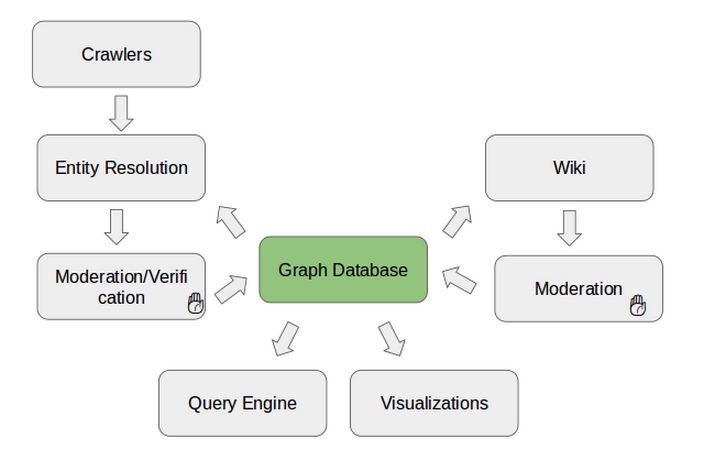
\includegraphics[scale=0.4]{tech_pic} 
\caption{Proposed System}
\label{fig:tech_pic}
\end{center}
\end{figure}

Components include:
\begin{itemize}
\item\textbf{Crawlers-Cleaner-Resolver} - As a part of the data acquisition module, the crawler crawls specific websites and scrapes data in format specified in a static file. Cleaner and resolver works on the scraped data. The cleaner makes the data more structured by keeping all data in specific format, discarding missing values etc. The resolver acts on the data to remove all duplicate entries (and merge similar entries) so to keep the data non redundant as possible.
\item\textbf{Verifier}- The data coming from the crawler after resolution is verified by human moderator. Any to-be-updated information is first human moderated. Any new data is then fed to the graph database.
\item\textbf{Graph database} - Acts as the data store for the system storing structured data with nodes as entities and edges as relationships.
\item\textbf{Web portal(Query Engine, Visualization, Wiki)} - This is the final product that is directly visible to the users. All visualizations (graphical, tabular) are done here. It also has an wiki interface for an end user to add more entities/relations to the graph database. The portal also includes a query/search engine to show results as per specific user queries.
\item\textbf{API} - Registered users can use this to read in data from the datastore in their application.
\end{itemize} 

%\section{SECTION NAME}
%\lipsum[2]


\chapter{System Pipeline}

%Replace \lipsum with text.
% You may have as many sections as you please. This is just for reference.
\begin{figure}[here]
\begin{center}	
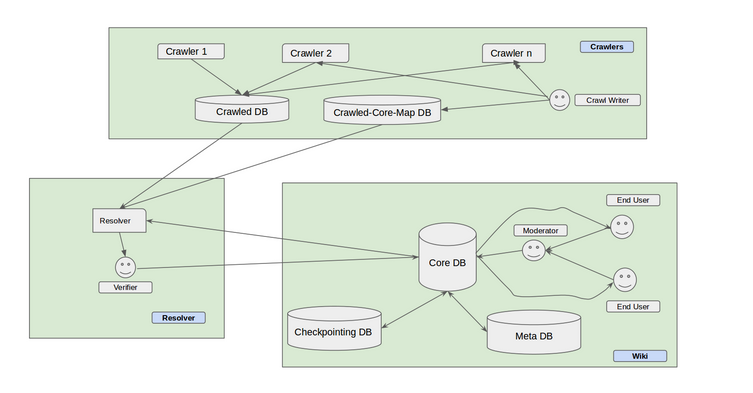
\includegraphics[scale=0.4]{sys_pipeline} 
\caption{System pipeline}
\label{fig:sys_pipeline}
\end{center}
\end{figure}
The total pipeline of the system can be seen in figure above. Overall, we have decomposed the system into 3 cohesive modules. In order of the data flow, they are - 
\begin{quotation}
Crawlers $\rightarrow$ Resolver $\rightarrow$ Wiki
\end{quotation}

\section{Crawlers}
%\lipsum[2]
This is the data acquisition module we have designed. Internally this module consists of the following components:

\subsection{\textbf{Crawler(s)}} - These are basically python scrapy/beautiful soup/selenium scripts to crawl particular websites and srape data from them. The nature of the data (i.e - data types, labels) is mentioned in the \emph{\textbf{Crawled-Core-Map}} database.

\subsection{\textbf{Crawled-Core-Map database}} - Contains the type of the data, its name(or label) to be scraped from a website. This mapping information is used by crawlers to produce output data of specific type,label. This map along with the specific crawlers are written by the developers (\emph{\textbf{Crawl-Writers}})

\subsection{\textbf{Crawled database}} - The raw output from the crawlers is written here. The schema of this database is largely dictated by the \emph{\textbf{Crawled-Core-Map}} database. The data is then read from this database into the \emph{\textbf{Resolver}} module.

\subsection{\textbf{Crawl Writers}} - They are the human components of this module. These persons are developers who write specific scripts to scrape desired websites. They are also responsible for maintaining the data schema in \emph{\textbf{Crawled-Core-Map}} database.



\section{Resolver}
%\lipsum[3]
This module works to fine tune the data scraped by the crawlers. All data collected thus far are mostly unformatted with duplicate or missing values. The function of this module is to process such data into a form suitable for the database.
Its constituents are:


\subsection{\textbf{Resolver}} - It takes the data from the Crawled database as input. The resolver can be further divided into two parts -

\begin{itemize}
\item\textbf{Cleaner} - The cleaner does the text normalization before the actual process for resolving begins. This includes out-of-format data, capitalization, missing-value issues which if not dealt with may cause the resolver to give low accuracy.
\item\textbf{Resolver/Duplicator} - Function of resolver is two-fold. Firstly, it checks any duplicate records in the incoming data (i.e. - data from the crawled database) and removes if any. Then, it resolves the entries from the crawled data with that of the core data. And outputs all possible matchings to the verifier for verification/tagging. 
\end{itemize}

\subsection{\textbf{Verifier}} The authenticity of the data should be checked before it can be inserted into the \emph{\textbf{Core Database}}.  The function of the verifier module and thus the human moderator is to tag the records outputted by the resolver module. These tagged records are the ones which are finally added to the \emph{\textbf{Core Database}}.


\section{Wiki}
This module is the web portal that is directly accessible to the end users. It consists of the interfaces that allow user to view, add, delete entities and their relationships interactively. 

\subsection{\textbf{Core Database}}
This is the main data store of the system. Care has been taken to ensure that whatever data goes in is redundant, free of noise and authenticated. \textbf{Neo4j GraphDB} \cite{Neo4j} is used in the backend for this. 

\begin{itemize}
\item\textbf{Why Graph database preferred here?}\\
Lot of brainstorming went in deciding to use Neo4j graph database. This is because a graph database stores the relations of records in the physical layer (unlike relational database) which makes faster retrieval of connections of entities without joins. And most of the analysis in social networks involves reading in the relationships/connections between entities. Hence query results can be produced faster here without any complicated joins.
\end{itemize}

\subsection{\textbf{Meta Database}} 
This contains the description of the data(format, source, type) being inserted in the database. This is especially useful when the data is authenticated against real-world information, so that every ounce of data in the core database is accounted for.
\subsection{\textbf{Checkpointing Database}}
Without a checkpoint, a Wiki is un-achievable. With every new update, a log of all changes is stored in this database. This is later used to roll back to a previous state to undo any new updates that occured. 
\subsection{\textbf{Web Server}}
Background server that hosts the web application currently has 3 major functions.
\begin{itemize}
\item\textbf{Wiki + Visualization} - The basic functionality of the web application is to provide the users with profiles and connections of organizations and personas which they can edit. The server also maintains a mechanism for checkpointing any data received.
\item\textbf{Query Engine} - To support the queries required for analysis of the network the server implements a query engine which takes queries of specific pattern and return results in tabular or visual format. This is achievable by Cypher query language which facilitates inquiring graph-like queries over Neo4j. These queries would go on the lines like: How are two entities connected? What is the shortest path between two entities? How far an influence of an entity goes over the graph? 
\item\textbf{Read API} - External applications can give GET requests to read data in json format. This aids research and analysis by end users.	
\end{itemize}
\subsection{\textbf{Others}}
Human components in the system - \emph {Users} and \emph{Moderators}. Users include the wiki-users who edit the Wiki to enter any new/updated info they have. They have to provide an evidential link for any information they commit.\\
The job of moderators is to verify records entered by users in the Wiki. They can be experts in their domain, they need to cross-verify from trusted sources.

\section{Example}
%\lipsum[2]
Here we describe how the Verifier and Resolver actually work with a working example.
\subsection{\textbf{Verifier + Resolver}}	
\begin{table}
\centering
\begin{tabular}{| c | c | c |}
\hline
{\bf Name} & {\bf Age } & {\bf Sex }\\
\hline
\end{tabular}
\caption{Sample data formats}
\label{table:1}
\end{table}


\begin{table}
\centering
\resizebox{\columnwidth}{!}{
\begin{tabular}{| c | c | c | c | c | c |}
\hline
{\bf Entity no. } & {\bf Graph label } & {\bf Graph props } & {\bf Mysql props } & {\bf Graph resolve props } & {\bf Mysql resolve props }\\
%1 & person & name,age,sex & name,age,sex & name & name \\
\hline
1 & person & name,age,sex & name,age,sex & name & name \\
\hline
\end{tabular}
}
\caption{Sample record of Crawled-Core-map database}
\label{table:2}
\end{table}

Let us say that the crawler crawls data and saves it in a format like in Table - \ref{table:1}
Also the crawler has an accompanying map-data information which looks like - \ref{table:2}\\
\emph{graph-props} column have one to one order wise mapping with \emph{mysql-props} column.\\
\emph{graph-resolve-props} column have one to one order wise mapping with \emph{mysql-resolve-props} column.\\

So, basically in the crawled data, each row represents a node with label :person and attributes (name, age, sex) in the core database.\\

\begin{enumerate}
\item Now, when a verifier logs-in a row from the \ref{table:1} is fetched, then \ref{table:2} is used to frame a query to search an entity with the name like in the row.
\item Matching nodes are suggested after the query to the verifier.
\item If verifier selects one of the propsed nodes, the resolved node is updated.
\item Else if the verifier doesn't find any matching node, a new node correspoding to the selected row is created and inserted in the core database.
\end{enumerate}

\subsection{\textbf{Wiki + Visualizations }}

\textbf{Profiles}\\

Following is a typical profile in the Wiki-

\begin{figure}[here]
\begin{center}	
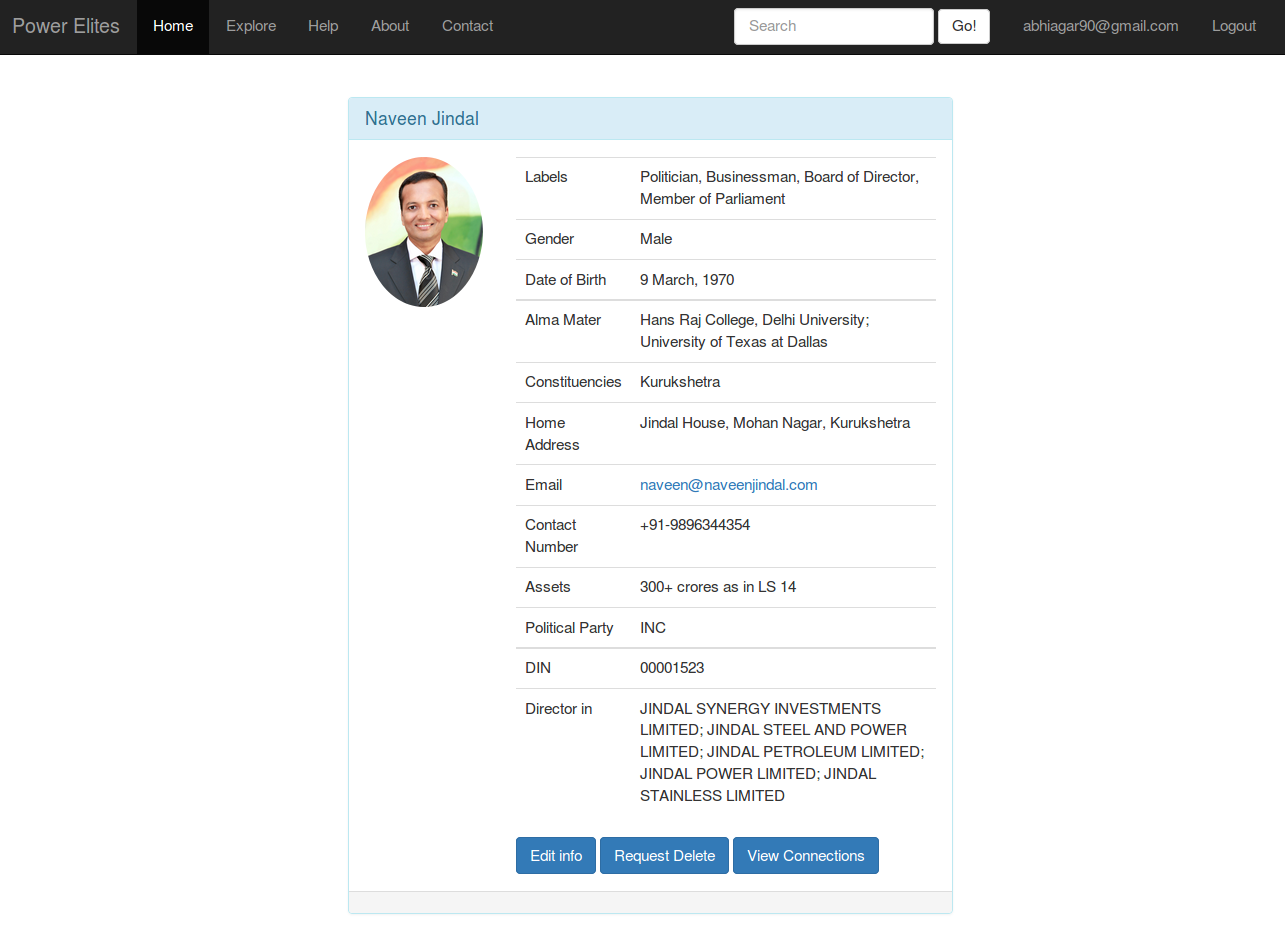
\includegraphics[width=\textwidth]{Jindal} 
\caption{Naveen Jindal Profile}
\label{fig:jindal}
\end{center}
\end{figure}

The figure above shows the Wiki page for industrialist Naveen Jindal containing information about him. It also contains interfaces for any registered user to edit as happens in a Wiki. It also allows the user to show connections of the person.\\

\textbf{Connections (Visualizations)}\\

\begin{figure}[here]
\begin{center}	
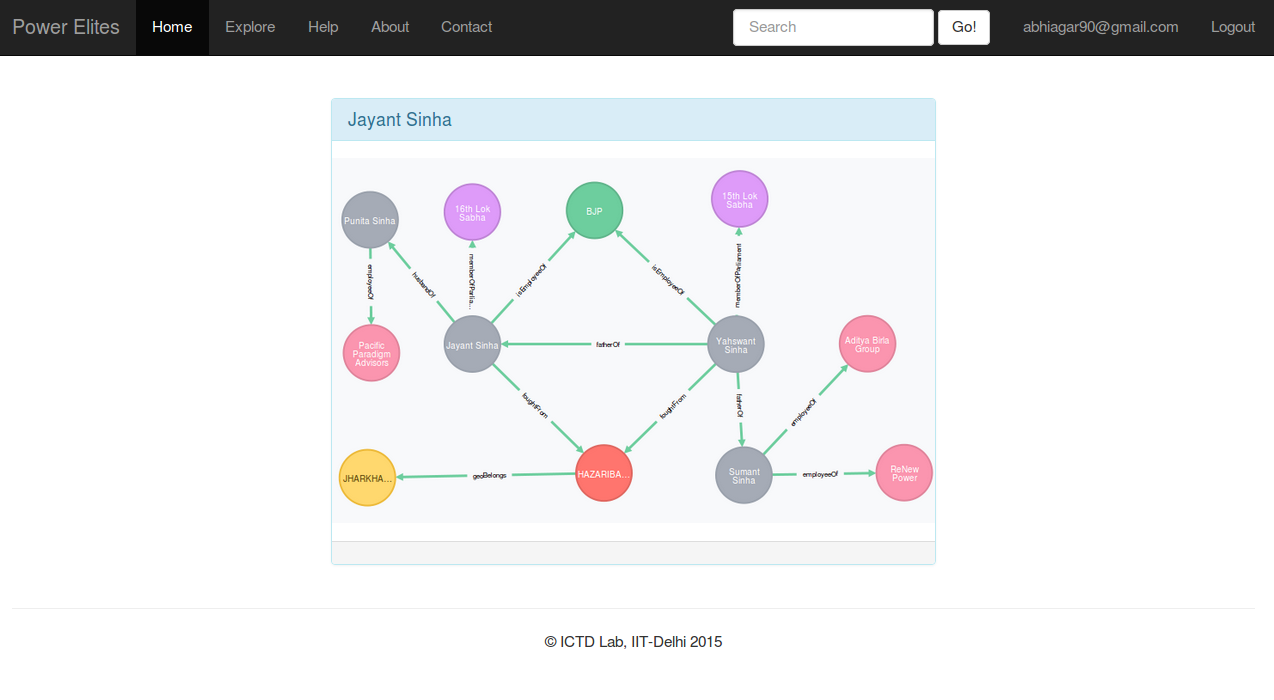
\includegraphics[width=\textwidth]{Sinha} 
\caption{Jayant Sinha Connections}
\label{fig:sinha}
\end{center}
\end{figure}
The figure above shows the connections for Minister of State for Finance Jayant Sinha. His connections include corporates firms like the \textbf{Aditya Birla Group} and \textbf{Pacific Paradigm Advisors} .

Other popular influence networks that our system shows is that of \emph{Gandhi Family and their Corporate linkups}, \emph{Jaydev Galla with his company with a large asset value}, \emph{Kamal Nath with Moser Baer}, \emph{Ravi Shankar Prasad with News 24 channel}.

\begin{figure}[here]
\begin{center}	
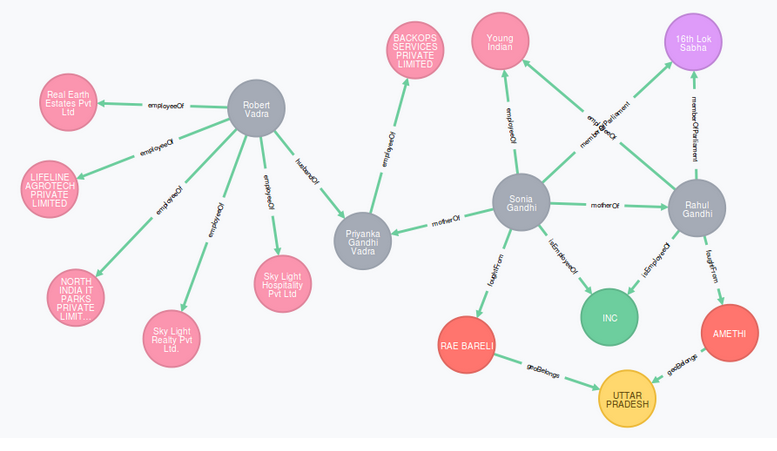
\includegraphics[scale=0.4]{Gandhi} 
\caption{Gandhi family}
\label{fig:gandhi}
\end{center}
\end{figure}

\begin{figure}[here]
\begin{center}	
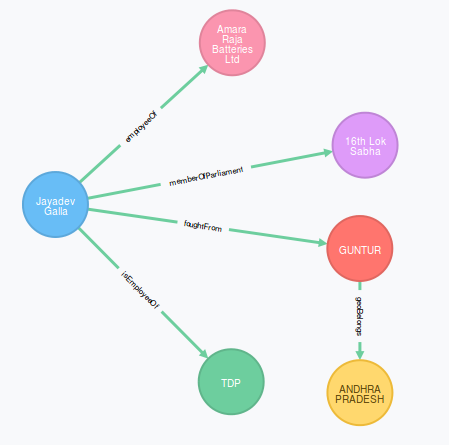
\includegraphics[scale=0.4]{Jaydev} 
\caption{Jaydev Galla Connections}
\label{fig:jaydev}
\end{center}
\end{figure}

\begin{figure}[here]
\begin{center}	
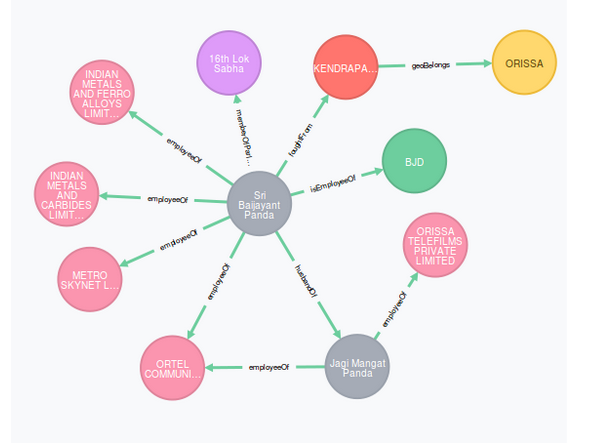
\includegraphics[scale=0.4]{Jay_Panda} 
\caption{Jay Panda Connections}
\label{fig:jaypanda}
\end{center}
\end{figure}

\begin{figure}[here]
\begin{center}	
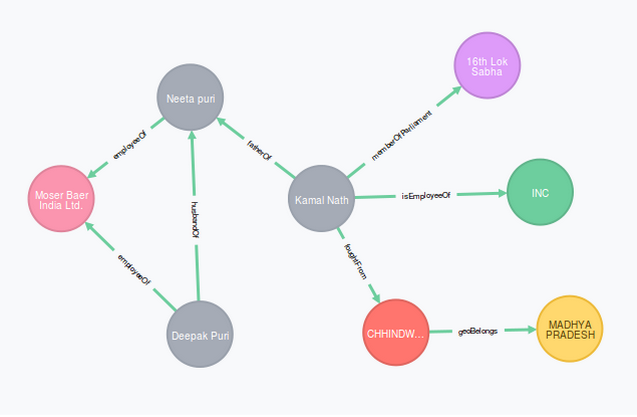
\includegraphics[scale=0.4]{Kamal_Nath} 
\caption{Kamal Nath Connections}
\label{fig:kamalnath}
\end{center}
\end{figure}

\begin{figure}[here]
\begin{center}	
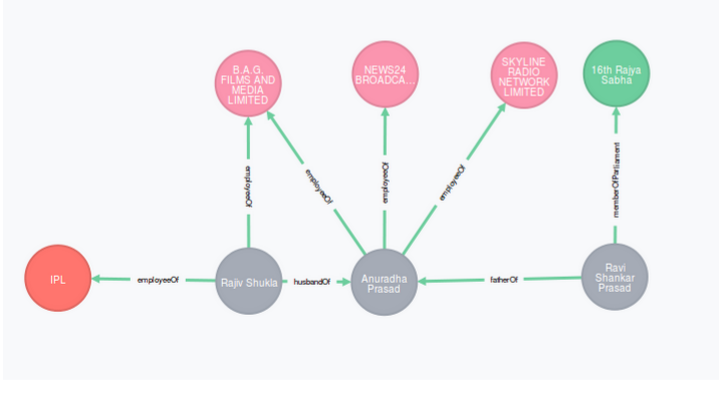
\includegraphics[scale=0.4]{Ravi_Shankar} 
\caption{Ravi Shankar Connections}
\label{fig:ravishankar}
\end{center}
\end{figure}



\chapter{Challenges}

%Replace \lipsum with text.
% You may have as many sections as you please. This is just for reference.

\section{Datasets acquisition}
Biggest challenge in mining political, bureaucratic, corporate data is the difficulty in getting relevant sources and structured information.\\\\
For our initial use cases we began by using political data from \textbf{MyNeta} \cite{MyNeta}. We plan to enrich this data from LokSabha and Rajya Sabha archives.
For corporate data, we used publicly available information from \textbf{CompanyWiki} \cite{CWIKI} and \textbf{Ministry of Corporate Affairs} \cite{MCA}.
As the system progresses we plan to include retired IAS/IPS officers, PPP data, family data of politicians, donations in our growing dataset. We already have about 1000+ politicians, 60000+ business people, 90000+ companies in our current core DB.  

\section{Data Modelling}
After getting some data the challenge was to model the data for the graph database. This would ensure listing of all possible entities and relationships of the system. Care was taken to form such relationships so that in the long run, queries supported by the system take optimum time to produce results.
The prominent entites(nodes) and relationships(links) modelled so far:\\\\
\underline{\textbf{Nodes/Entities}}-\\
(\textbf {Person} (uuid, name, address-location, DOB))\\
(\textbf{Politician} (uuid, name, mynetaid-electionname-year, constituency))\\
(\textbf{Alias} (uuid,name,context))\\
(\textbf{Party}(uuid,name,type:\emph{"national,state,regional"},start-year,HQ))\\
(\textbf{Company}(uuid,cin,name,location,income,expenditure,profit,value))\\
(\textbf{IAS} (uuid,name,DOJ,year,IAS-ID,posting-location))\\
(\textbf{Employee}(uuid,din,name,designation))\\
(\textbf{Govt-Body}(uuid,name,location))\\

\underline{\textbf{Relationships/Links}}-\\
(\textbf{Politician})$\rightarrow$(\textbf{member-of}(id,type,years)$\rightarrow$(\textbf{Party})\\
(\textbf{Politician})$\rightarrow$(\textbf{member-of}(id,type,years)$\rightarrow$(\textbf{Govt-Body})\\
(\textbf{IAS})$\rightarrow$(\textbf{member-of}(id,type,years)$\rightarrow$(\textbf{Govt-Body})\\
(\textbf{Employee})$\rightarrow${employee-of}(id,designation,years)$\rightarrow$(\textbf{Company})\\
(\textbf{Company})$\rightarrow${donated}(id,cin,party,amt,year)$\rightarrow$(\textbf{Party})\\
(\textbf{Person})$\rightarrow${family}(id,is-biological$\rightarrow$(\textbf{Person})\\
(\textbf{Person})$\rightarrow${profession}(id,type)$\rightarrow$(\textbf{Politician})\\
(\textbf{Person})$\rightarrow${profession}(id,type)$\rightarrow$(\textbf{Corporate})\\
(\textbf{Person})$\rightarrow${profession}(id,type)$\rightarrow$(\textbf{IAS})\\
(\textbf{Person})$\rightarrow${aka}(id)$\rightarrow$(\textbf{Alias})\\

\section{Latency and Optimizations}
Although implementation of basic system is ready, its performance suffers when single GET request to the Web server calls for multiple read requests to the core database. We are planning to alleviate this problem by indexing the database to optimize search time, forking multiple threads.


\chapter{Epilogue}
%TODO - expand the questions
\section{Conclusion}
 In short what hypothesis you predicted before starting to build the system?? Do you find them in the results?? Any other interesting patterns?? 
What else can you conclude from your work?? What are your conclusions from the data collection stage? How and why is it difficult to get Indian data?? Did the data model worked well with graph db ?? Is it possible to resolve entities from two different datasets and find interesting connections??  What did your system show after data mashup?? How practical is your system taskflow if deployed in real world??

\section{Future work}
%\lipsum[2]
We have tried to start a process of building a system which in the long run will help the Indian society. Our best efforts were to cover up as much functionality as possible. Yet however, many other problems or features are left to be done in future.
%TODO - expand the questions
\begin{itemize}
\item Scaling up - The designed system works fine. How the system would scale up? How to handle more data when it is fed to the system?
\item Better Visualizations - Can the visualizations be saved/ annotated/ more interacting??
\item Inference Engine - Can the inferencing process be automated? Like in expert systems which uses a knowledge base and Prolog scripts to produce more knowledge??
\item Better analysis of Social Networks - can the different questions about the social graph be answered? What about degree centrality?? No. of weak ties?? Clusters and their strengths? Can we compare with the random graph model to produce some interesting social network behaviors ??
\item Better Query Engine - Can the query engine be improved so that even users not knowing CQL can give queries?
\item Other use cases - Can other data be looked to expand the network with more nodes and relations?? What about IAS officers?? Monetary donations?? Media ownerships??
\end{itemize}


\chapter{Amartya Rough}

\section{Entity Resolution}
The basic algorithm of entity resolution goes as follows-

\begin{algorithm}[H]
\KwData{Datasets - S, T }
\KwResult{list -L consisting of proper matches of T in S }
initialization - L is empty \;
parameters - S,T, threshold \;
 \For{all records in t in T}{
  \nl search for t in S \;
  \nl pick records s in S for which match-score(t, s) $\geq$ threshold \;
  \nl append s in L \;
 }
 \caption{Basic Entity Resolution}
\end{algorithm}

Complexity of above algorithm is O(n*m) where n is size(S) and m is size(T) when n records are searched linearly in S.
        From the above, we can find that the two crucial operations here is the choice of proper scoring algorithm to pick s and search of t in S in line [line].

\section{String Matching Algo}
        The requirement of a scoring algorithm was such that it should match words with small spelling mistakes and similar names. In our case, we have used Jaro distance as it considers ranges and transpositions while matching two words. A sample experiment from our side on a list of four names showed the following scores - 
        [[tble]]
        Upon a test run of all algorithms over a sample of 100 names from our datasets we decided to use jaro-winkler for the purpose. We also required to match names which are phonetically similar to other names. These helped us to match names like 'Gautam' and 'Gautambhai', 'Vidya', 'Bidya' and 'Viday' etc.

\section{Comparison techniques}
        As obvious from above algorithm the performance of entity matching algorithm depends largely on how fast the searching occurs in dataset S. A naive algorithm like above added a factor of O(n) on linear search over entire S. The obvious improvement over it is the possible implementation of a binary search to reduce search speed to O(log n) time. But binary search is not applicable here for following two reasons -
            - Binary search uses a predicate like gt, eq, lt , the value of which is true or false. Such predicates determines some order in the dataset. 
            - The absence of such predicates as above avoid any sorting or ranking of the data in any order.
        As a result, the performance of the entire system got bottlenecked by the resolution module. As a result we sought out for other solutions regarding this.

\section{Machine learning techniques}

        After having performance bottleneck in searching records in other datasets, we looked for probabilistic ways of solving the same problem. We used the python library of csvdedupe for this purpose. The library basically induced an active learning mechanism to obtain training samples where it picked two entities of possible match and prompts the user to label positive/negative. It then matches the related entities accordingly with the hypothesis formed. Unfortunately this approach suffered from following drawbacks-
        \begin{itemize}
        \item Too small data to accurately form a proper hypothesis. 
        \item The labels that were asked to mark alongwith data were picked at random and often the results of the algorithm are different in different runs (depending on the number of positive or negative label given at that time).
        \end{itemize}
        Fortunately indexing other dataset helped to come out of this.

\section{Indexing and Apache Solr}
        Indexing allows searching to be very fast of near O(1) speed. Indexes are datastructures that store contents of a document (in our context fields of records in a dataset) for faster access to the document. This enables faster retrieval with a trade off for using more memory. For our purpose we used Apache Solr framework for the searching step.Solr uses Apache Lucene to create an inverted index based desired on fields in the records. An inverted index basically creates a data structure on the content of the records and have pointers to the actual locations of the records. So for all text in the specified fields, Lucene breaks them (tokenizes them) and store them in a data structure for fast retrieval.  Solr also sets up a  Web server with REST APIs to allow us to integrate it with other parts of our system described in chapter [give reference here]. 
        Since Solr has its own sets of protocols we had to modify the way we apply the resolution algorithm described above. The main steps followed by us to realize this are as follows. 

        - Defining a data set to index  (the data set S above). We described a data source which contained the dataset. In this case, it was a mysql database. (file db-data-config.xml) .
        - Defining the fields to index. Solr needs to have a schema of the records to know which fields will indexed and which one is kept as satellite data. These are specified in solr configuration files. (schema.xml)
        - Defining how to preprocess all the terms before creating the index. Solr allows to specify a list of pre-built tokenizers, stemmers, filters to preprocess a term or custom ones if necessary. We used whitespace tokenizers and double metaphone phonetic filters to get a match score relevant to our purpose and in this way used the phonetic algorithm for better text matching. (file - solrconfig.xml)
        - Forming a lucene query based on the contents of records of another dataset (data set T above)
        - Applying Jaro algorithm for comparison was difficult in Solr. This is because, all the functions applied to the text for indexing are necessarily single parameter. Jaro or any other non-phonetic string metric needs at lest two string Results returned by the Solr is further filtered by the Jaro-Winkler algorithm. Results being quite small, does not take much time even if a one-one matching algo is executed. 

\subsection{Solr Fields}
    To effectively triangulate two entities, special emphasis was given on which fields to compare while doing it. After few experiments we decided to match records on following fields generated from the graph data model we discussed in previous section.

    - Aliases - a list that contains names pertaining to an entity. This is especially required when a person/institution is known by several names in the world. Eg. - Narendra Modi vs Narendra Damodar Modi, BJP vs Bharatiya Janata Party 
    - Aliases Phonetic - same as above but here search is done on phonetic index.
    - label - Label dictates the type of entity as per data model in chapter [refer chapter here].
    - Keywords - a list that contains main keywords of the entity. This field is most helpful in triangulation as it indexes all the properties of the entity and the aliases of the entities directly related with the original. Important properties unique to a particular entity like location for a particular item.

\subsection{Lucene Queries}
    Proper search queries are essential to effeciently resolve an entity. These involved using above fields effectively to obtain relevant entities- 
    The grammar of the lucene query used by us goes as follows-

    L:= I:(Q) AND L OR epsilon

    where I is the index field (one of above) and Q is the query string to be matched against I
    Where index field is one of the above and query string can be as follows -
    "string text" - matching the exact word 'string text'
    string text - matches string or text or both
    string~ - lucene applies edit distance to string and returns the possible matches

    The query we used for our purpose is as follows-
    " labels:(each label separated by whitespace) aliases:(each alias~ separated by whitespace ) AND aliases-phonetic:(each alias separated by whitepace) AND keywords:( each keyword~ separated by whitespace)"

    Eg. - 
\subsection{Performance}
    On testing our Solr integrated system with the original basic resolution algorithm, we found many fold improvements. Initially upon resolving 1000 corporate entities against about 500 political ones over the "name" field in both took us about 150 minutes to resolve. That makes resolution of a single entity about 18s.
    Compared to that, a single entity is resolved in Solr in little over 1s showing a performance upgrade of about 18x.






\chapter{Constructing the Social network}

The driving fuel for any social network is the data it represents. The problem in constructing a linked-data system such as this one is always the data and the entropy it brings with itself. The challenges are always the usual ones - unavailability of data, noise in the collected data, no authentic source, and many-a-times no structure in the data. Even if we are successful in collecting and cleaning the linked data we want, the way we go about integrating all this variety of information in a single data store is itself an another challenge. \\

The choice of data store matters here the most because one would like to query the data and unearth interesting relations between participating entities. Henceforth, a person or an organization will be called an entity. These entities would be linked to each other by certain edges/links just like in a graph which we will normally call relations. All these challenges are elevated manifold when one wishes to resolve entities from different datasets into a single unified entity. \\

Here we describe in order our choice of data storage, our core data model for the linked data, data collection practices and data sources, data integration methodology, and finally the necessary evil in such a system entity resolution. \\

\section{Everything is a graph}

We begin by describing how we are going to actually store any kind of linked data we get and why our approach is a sensible one. We describe here where our core data is stored and how our core data model looks like. It has to be stated at the onset that care has been taken to ensure that
whatever data goes in our core data modal is non-redundant, free of noise and verified. As already stated, our goal is to construct a social network between politicians, companies, entrepreneurs, military personnel, bureaucrats, political parties, universities, movie actors, and any important entity one can think of in the usual power hierarchy. Also, we want to be able to model all kinds of relationships that can exist between these entities with ease: family-links, donation-links, director-links, ownership-links, subsidiary-links, etc. \\

Practically anything connected can be represented by a graph(or a hyper-graph to be exact, refer our LIMITATIONS section). We live in a connected world. There are no isolated pieces of information, but rich, connected domains all around us. Thus, it makes sense to model our core data as a large inter-connected graph where every node is an entity and every edge represents a link between two of them.   \\


A graph is composed of two elements: a node and a relationship. Each node represents an entity (a person, place, thing, category or other piece of data), and each relationship represents how two nodes are associated. This general-purpose structure allows you to model all kinds of scenarios – from a system of roads, to a network of devices, to a population’s medical history or anything else defined by relationships. [https://neo4j.com/developer/graph-database/]

Before beginning to describe how we achieve the above, it is important to understand that even traditional SQL tables are a connected piece of information, and can be modeled using a graph. \\

What we provide is therefore a graph to the user where he fits any relevant connected data he has. The choice of the data model is clear, but two problems remain - how we are going to store our graph's interconnected data, and how do we query it efficiently for digging out interesting relationships. Our next two sections discuss the same. \\

\subsection{Neo4j}

Neo4j [https://neo4j.com/] is our choice of data storage. It is one of the leading JVM based NoSQL graph databases. We build our knowledge base on it as a graph and thus Neo4j is at the center of our entire system. We chose Neo4j because of the following reasons[https://neo4j.com/developer/graph-database/], and we have found it be a non-separable asset to our use cases. \\

\begin{enumerate}

\item Only a database that embraces relationships as a core aspect of its data model is able to store, process, and query connections efficiently. While other databases compute relationships expensively at query time, a graph database stores connections as first class citizens, readily available for any “join-like” navigation operation. Accessing those already persistent connections is an efficient, constant-time operation and allows you to quickly traverse millions of connections per second per core.  [https://neo4j.com/developer/graph-database/]

\item Graph databases are designed to mimic the most natural way we tend to model data – the same way you would map it all out on a white-board. Your collection of circles, boxes, lines and arrows is – in essence – already a graph. [https://neo4j.com/blog/graph-data-modeling-success/]

\item In Neo4j, everything is stored in form of either an edge, a node or an attribute. Each node and edge can have any number of attributes. Both the nodes and edges can be labeled. Labels can be used to narrow searches. [http://neo4j.com/docs/1.8.3/indexing.html] Neo4j is very easy to learn and adapt. It's object property model is very intuitive and anything can be modeled on a white board in the form of nodes and edges.

\item Constant time traversals for relationships in the graph both in depth and in breadth due to efficient representation of nodes and relationships [https://neo4j.com/developer/graph-database/]

\item All relationships in Neo4j are equally important and fast, making it possible to materialize and use new relationships later on to “shortcut” and speed up the domain data when new needs arise [https://neo4j.com/developer/graph-database/]

\item Compact storage and memory caching for graphs, resulting in efficient scale-up and billions of nodes in one database on moderate hardware [https://neo4j.com/developer/graph-database/]

\item It's NoSQL help us in modeling the varied data from different sources we have collected.

\item The cypher query language provided by Neo4j helps in querying the connected data very easily and is very powerful. Also, the Neo4j browser client provided by Neo4j is vary good for visualizing the results of the cypher queries.

\end{enumerate}

That said, it is important to note that Google uses Cayley - an open source graph database -  to power it's google's knowledge graph. [citation: https://github.com/google/cayley] 


\subsection{Property Graph Model Explained}

Let us dive into some examples which explain how me model our core data in Neo4j using it's property graph model. [https://neo4j.com/developer/graph-database/] \\

\begin{enumerate}

\item The property graph contains connected entities (the nodes) which can hold any number of attributes (key-value-pairs). What this means for us is: a person node can have different attributes his date-of-birth, address, email, sex, etc.

\item Nodes can be tagged with labels representing their different roles in our domain. That said, this unique thing about Neo4j helps us in specifying IS-A relationships via multiple labels on a single Neo4j node. Thus, a node can be labeled as a person, politician, businessman at the same time. The same information is very hard to model in traditional SQL databases.

\item In addition to contextualizing node and relationship properties, labels may also serve to attach meta-data index or constraint information to certain nodes.

\item Relationships provide directed, named semantically relevant connections between two node-entities. A relationship always has a direction, a type, a start node, and an end node. This model is exactly the same as directed edges in a traditional graph structure. Although they are directed, relationships can always be navigated regardless of direction.

\item A relationship can also be labeled by a single label specifying what kind of a relationship exists between two nodes. Thus, if a politician is 'son-of' a businessman we can connect the two nodes by an edge attributed with such a label.

\item Just like a node, a relationship can also hold any number of attributes(key-value pairs). In most cases, relationships have quantitative properties, such as weights, costs, distances, ratings, time intervals, or strengths. But for our use case, one can think of an example relationship as : a particular `person`(node) 'donated'(relationship-type) 'x amount of money at y date'(relationship properties) to(directed edge) a particular `politician`(node).

\item As relationships are stored efficiently, two nodes can share any number or type of relationships without sacrificing performance.

\end{enumerate}

An example could be the image [image 1]

\subsection{Cypher}

Cypher is a declarative graph query language for the graph database Neo4j that allows for expressive and efficient querying and updating of the graph store. Cypher is a relatively simple but still very powerful language. Very complicated database queries can easily be expressed through Cypher. This allows users to focus on their domain instead of getting lost in database access.[http://docs.neo4j.org/chunked/stable/cypher-introduction.html] \\

A node is represented like this: (:person:politician {name:'Narendra Modi',sex:'M'})
A relation is represented like this: (startnode)-[:relatedto {kind:'childof'}]->(endnode)
The structure here is self explanatory and can be further explored by reading Neo4j manual. A sample image[2] here describes the image for cypher.


Querying in cypher is as easy as thinking about how you traverse a graph. Here is a simple query to return all the relationships that start from or end at node 'Naveen Jindal' of type politician.

MATCH (jindal:politician {name:'Naveen Jindal'})-[anyrelation]-(anynode)
RETURN anyrelation

Interested readers can be direct here to read more about cypher in Neo4j's manual: [https://neo4j.com/docs/developer-manual/current/]

\subsection{Our restricted property graph model}

We had to specify some ground rules to model our data for imposing uniformity on varied data that is being fed into the system. Thus, our property data model follows the rules stated below.

\begin {enumerate}

\item As allowed by Neo4j - a node can have more than one label, a relation always has only one label.

\item Every node and a relation has a unique uuid/relid

\item All nodes are labeled 'entity' by default. To make anonymous queries on nodes easier.

\item All living or dead people are labeled 'person'.

\item Any person connected to a company as a director/owner is labeled 'businessperson'.

\item All operating units are labeled as 'organization'.

\item All companies is labeled as 'company'

\item A political party is labeled as both 'organization' and 'company' alongside 'entity'

\item Other self-explanatory labels for nodes in current core data are: city, state, constituency.

\item Every 'entity' will have to have a name property. An aliases property - a neo4j array - helps in keeping track of different names of an entity.

\item An 'entity' can have any number of properties, but these properties if present are validated: 'startdate'(int), 'enddate'(int), 'iscurrent'(boolean). For a person a 'startdate' represents his date-of-birth, for a company 'startdate' represents it's incorporation-date. The 'iscurrent' property can help us in tracking if the 'person' is dead or the 'company' is not active.

\item startdate and enddate are timestamps since epoch - so any date-of-birth or company's incorporation-date will have to be converted to a particular format before pushing to the system.

\item All relationships have to have a property bidirectional - to explicitly specify if the relationship goes both ways. This had to be done as Neo4j edges are always directed, though they can be queries without directions.

\item  Some labels for relationships in current core data are: relatedto, worksin, geoBelongs.

\item An entity can have any number of properties, but these properties if present are validated: startdate(int), enddate(int), iscurrent(boolean). For a person a startdate represents his date-of-birth, for a company startdate represents it's incorporation-date. The iscurrent property can help us in tracking if the person is dead or the company is not active.

\item All the other meta-info will be stored in a separate sql database that will help in mapping any data point change to it’s source and the user who allowed that change. this is better explained in the provenance section in system design chapter.

\end{enumerate}

We list some images here that better describe the present data model. [all the model images]


\section{Data collection and description}

Since the aim was to to build a social network for all the Indian power houses, we needed to identify and collect as much varied data as possible. It is only when different kind of data mingle with each other in the system that we can hope to see some hidden patterns or dig out interesting insights. All the visualizations that we obtained from this data is shown in the analysis section. [citation]

We needed to search for alternate data sources that might help the ongoing work. We have looked for datasets spanning company details, board of directors, Lok-Sabha MPs, subsidiaries, banks, and any other relevant political-corporate data. 

Any data that is crawled is not fed into the system directly. Instead, a REST PUSH api provided by our system is used to push it to a separate crawl data-store (rather than the core data-store) for moderation first. The  data integration is described in next section, while the rest api is described in next chapter. [citation]

\subsection{Challenges}

\begin{enumerate}

    \item  The biggest challenge in data collection is that data for Indian context is not easily available.  Open data initiatives like data.gov.in have initiated hope for data enthusiasts but there is still a long way to go. [citation]

    \item No central place for any category of target data, so one would have to look for multiple sources. Instead, in a way, we are striving to create such a central place in the present work.

    \item Since data has to be integrated from variety of source points, the credibility of a data item listed can be established strongly but with the added evil of entity resolution - which has been explained in a later section [CITATion section]

    \item Mostly, no unique identifiers for entities appear in datasets that are publicly available. There is a possibility of duplication of data, this is where the ER work comes in handy. [citation] 

    \item Most data contained noise, or erroneous details at times. This sometimes is intentional on the data entry operator's part, sometimes it's just a naive mistake. For example: name for some people was wrongly spelt in some publicly available websites.

    \item Data was missing for some datasets. For example, in the affidavit that the politicians have to fill before elections, or in the data collected from companywiki.

    \item Names are the biggest problems in such a work. People use titles like Mr., Shri, Shriman, Late, Lt., Mrs., Kumari, Kumar which again add more complexity to the problem. 

    \item There is no standard data format for dates even across government departments. Similarly for the address - there is no standard format to extract out relevant information.

    \item Most of the government sites maintain significant data on-line but hidden in a complex web of links and they love uploading data in PDFs! 


\end{enumerate}


\section{Tools and Methods}

We describe here tools that we picked up along the way for data collection and data cleaning. It is important to note that no single tool can be a cure for all the data-sources. In fact, what we have learned in due course of time is that different kind of data sources require different approach.

[todo]

\begin{enumerate}

    \item A naive method that we experimented during the initial work is to fetch a source url through python's urllib library, and then process it using BeautifulSoup. 

    \item selenium

    \item scrapy

    \item manual at times: if data less and useful for connections. 

    \item data collected is preprocessed using pandas library, nameparser, wote our own algorithms for converting date-of-birth to startdate format (int) -  timestamp epoch

\end{enumerate}


\section{Corporate data}

The challenges in collecting any corporate data are:

\begin{enumerate}
    \item Getting government provided unique identification numbers for the company
    \item Getting government provided director identification numbers for their directors
    \item Linking these two IDS.
    \item Getting the list of all companies over the time with their Ids of course.
    \item Getting the list of subsidiaries for each company/group. (The toughest job)
\end{enumerate}  

[todo]
We have been able to tackle the first four challenges to a commendable extent but the last one. A related work is Parag's [citation]. We first describe the sources we have encountered, and finally how we collected our corpus of 60000 directors and 90000 companies.

\subsection{MCA}
[citation mca]

Being the official government source, this is the most authentic data source we have found for obtaining the list of companies and LLPs (Limited Liability Partnerships) operating in India. It gives us all the companies registered year-wise before and after 1980 till date in the form of pdfs with their CIN/LLPIN (Corporate Identity Number/Limited Liability Partnership Identification Number) which is unique to a company/LLP. The only downside as always with any pdf data is a lengthy parsing job.

MCA, with its search engine, is amazing! Armed with the CIN, we can obtain a lot more information for a company from the MCA site itself. We get the type of the company, the category of the company, the headquarters, its market capital, date of incorporation and the charges it is facing. Not only that we also obtain the signatories of a company from the MCA site as well i.e. their board of their directors, with their unique DIN(Director Identity Number). This can again be useful in entity resolution. (This is a new feature they introduced).

[todo: mca problems
crawl: why not
]


\subsection{capitaline database}
[ciation cpaitaline]
One of the main challenges was to figure out the subsidiaries of a firm. This would complete the picture of the company network. Alas, finding the subsidiaries is not an easy task. We could find just one source after running around all over the internet:  Capitaline. However, the data seems to be spotty at best. We could not find details for a lot of the listed subsidiaries.

The problem with capital line is multifold: No CIN, LLPIN. Very bad interface to crawl but nonetheless crawlable. It has no single source of the companies. And subsidiaries information extraction would just reveal names of subsidiaries, no unique IDs! There is no hyperlink from the subsidiaries name to any company page.

Parag has already collectd this data [citation] todo



\subsection{companywiki}
[citation compnywiki]
[todo]
advantages
linked data
reverse search from both directions
seed parag dataset
three days crawl selenium
dataset stats
linked data
our core base


\section{Political data}

ls crawl from ls site - images too - 

Our task in this domain was to find personal information of MPs and their dependents. So we went looking in Wikipedia of various political members and their families. But Wikipedia is highly unstructured and crawling, parsing Wikipedia even with professional extractors is a tedious task.

We started with these problem statements in our mind:

How to get info on all 16 Lok Sabhas’ MPs?
How to get the family information of MPs?

\subsection{MyNeta}

they have done a tremendous work in digitizing this data
courtesy
data description
problems -  missing fields, name format
info about constituency and states 
info about assets and liabilities
info about criminal cases
mynetaid for a particular election helps in resolution from myneta dataset, kept as internal prop
ls 2009 and ls 2014 data

\subsection{Lok Sabha Official data}

describe how we got the data
name and address problem
why we choose the data gain when we had myneta- family links of politicians


\subsection{Rajya Sabha Official data}

describe how we got the data
name and address problem
why we choose the data family trees of politicians




\section{Family data}

why to see if somehow the powerhouses are connected 
known examples already include naveen jindal, jayadev galla, etc.
chidambram and his family in news already, etc.
[citation: https://en.wikipedia.org/wiki/Category:Business\_families\_of\_India]
[citation: https://en.wikipedia.org/wiki/Political\_families\_of\_India]

All the mash-ups created by these datasets have been reported in viz section. [citation: viz section]

\section{Data integration}

[TODO]

Many data sources, many data-gatherers, different kind of data
We describe here : How do we integrate all into one unified model described above
Though the system has been described in detail in later section, we felt that our data integration model should be described here - data integration is a major challenge - and it is one of the major breakthrough that we did while designing the system \\

The idea is to keep data-collection part separate from the system - separation of concerns
What this means is data-gatherer cannot share any data stores with the system
They basically push their crawled data to the system using REST api with a json payload
The system doesn't know about how the data-gatherers are crawling and storing their data or the schema of their data, or where they are storing the data,  the system doesn't need to know if the data-gatherers run their scrapers and crawlers regularly
The rest api calls will be authenticated which is described in system design section [citation] \\

Initially, we were planning to open a mysql data-store with a fixed schema for the data-gatherers to directly write to. We planned separate tables for each of them and mapping tables to describe each row. As bas as this design sounds, it would have been an expensive mistake in the long run. \\

The present system communicates with all the data-gatherers using json. Why json? It is the new language of the web, mingles well with language like python, and is non-structured - exactly what we need to support our core data model - similar to a NoSQL schema. JSON (JavaScript Object Notation) is a lightweight data-interchange format. It is easy for humans to read and write. It is easy for machines to parse and generate. [citation : json.org]   \\

the json payload in the rest api is such: along with the authentication information(described in system design section): it has two json array objects : entities and relations. \\

entities array contain description of the entities in the freshly pushed data - almost like in Neo4j. 
it has five variables : id, sourceurl, labels, properties, fetchdate - id is unique identifier for the node for that data-gathering task. note here that labels and properties here  - sourceurl, fetchdate will be used for provenance as described in later section \\


Since we need every data to be accounted for ---  sourceurl and fethdate
gatherers will know the source and when the data was fetched 
[citation: sample screen shot of json entities payload] \\

relations array contain description of the relations between the entities discussed above 
it has eight variables : id, sourceurl, label, properties, fetchdate, start\_entity, end\_entity, bidirectional - id is unique identifier for the relation for that data-gathering task. note here that label and properties here  - sourceurl, fetchdate will be used for provenance as described in later section -- bidirectional is the necessary relation property that we described in data model section---start\_entity and end\_entity are foreign key references to the unique ids in entities array.  
[citation: sample screen shot or code listing of relations payload] \\

all data crawled or manually collected is first pushed into crawl data store (aka crawl-DB) -  another separate neo4j database -  using rest api calls over json payload -- 
This way - we will have different non-connected subgraphs in the crawl data store(again a neo4j db).  
But how do we resolve the nodes and relations now with the core data store? The basic setup id described in the next section. \\


\section{Data resolution}

here

\chapter{Detailed System Design}

In the present chapter, we dissect our system bit by bit and describe each component in detail. We have already described how our data is integrated from different data sources, and also how our ER system works. Here we describe the wiki and the web app that uses all those features.  It is important to note that our sole aim while designing the web application (and the entire system) was to reduce manual work of the verifier - so a lot of brainstorming and design changes went in that direction. Any feature or performance improvement in the verification process makes life easy for the verifier. The system has been designed to be able to crowd-source the verification process like others. \\

Another key point which we have kept in mind always while building the system is to make the 
data-gatherers task hassle-free  - that they should universally be able to communicate with the system. Towards this effect they should also be able to keep track of their data, and also update their old data as well. We have already described how we achieve this using json and rest over a Neo4j back-end we call crawl data-store. We have already described how separation of concerns  further help in achieving this as the crawled-data is well separated in crawl data store. \\

\section{Terminology}

\begin{figure}[H]
\begin{center}  
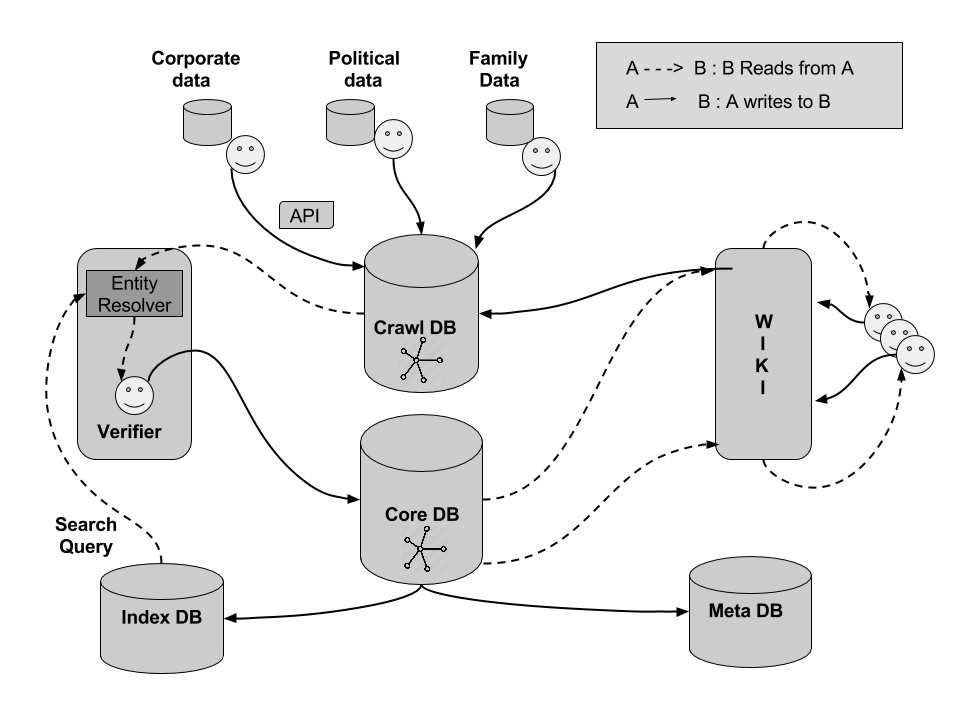
\includegraphics[scale=0.3]{system}
\label{fig:system}
\caption{Detailed Design}
\end{center}
\end{figure}

The detailed design of the system can be see in \ref{fig:system}. We formally define the terminology about the actors and system components here:

\begin{enumerate}
    
    \item Data-Gatherer: An authorized individual or a group of individuals who crawl linked data from different sources. This data can be about entities and relations that belong to any domain supported by our system: political, corporate, sports, bureaucratic, etc. A data-gatherer can use their API-token to push data to our crawl data store using json payload.

    \item Crawl Data Store: The Neo4j data store which stores all non-verified, non-resolved data that data-gatherers push into the system. All data from here is first verified and resolved  

    \item Resolver: A tool that searches over indexed graph data to suggest possible entities for a given entity. ER mechanism has been described in previous chapter in detail. A resolver in essence in our system suggests the probable matches but does not resolve.

    \item Verifier: An authorized person (or a bot) who matches an entity against a possible list of suggestions by the resolver. The only human element on which the system is dependent to be able to push data to the core data store.

    \item Core data store: The Neo4j data store which stores all verified, resolved data that data-gatherers push into the system.  This basically represents our knowledge base - a potpourri of data from different sources.

    \item Registered User: An authorized user who can use wiki to suggest changes to an entity or a relation in the core data store. All these changes are directed to crawl data store.   

    \item Wiki: Part of the web app, where registered users can edit or add information to the core data store.

    \item Meta-DB: MySQL back-end which stores provenance of any info added or changed in the core data store.

    \item Index-DB: MySQL back-end which stores condensed information (and connected information) of all the entities in the core data store. Apache Solr runs on top of it to index this information to help the resolution process. 

    \item Admin: The user with all the privileges in the system - can also delete all indexes, refresh all indexes, see which user/verifier contributed most to the system, change roles of a user.

    \item End user: Non-authorized users that can access information through the web app. They cannot make or suggest any changes to the core data store.

    \item Role: All the authorized users in the system are given a role. The roles are in scoping fashion. The role order from the top is as follows: Admin, Verifier, Crawler, Registered User, End User.  

\end{enumerate}

We have described the tech used in the system in the appendix section. [TODO: did we??]



\section{Data Gatherer}

The use case diagram for data-gatherer is shown in Figure \ref{fig:gatherer}.

\begin{figure}[H]
\begin{center}  
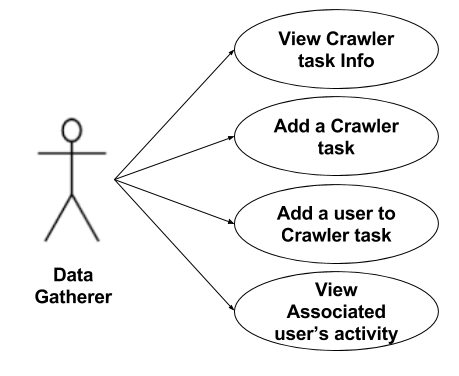
\includegraphics[scale=0.3]{gatherer} 
\caption{Use cases for Data Gatherer}
\label{fig:gatherer}
\end{center}
\end{figure}


\subsection{Task creation}
A group of data-gatherers are assigned a unique task identifier when they create a task for their crawled data \ref{fig:taskcreate}. This helps in separating the data from different tasks, due to which the crawl data-store has different disconnected subgraphs. The data-gatherers can keep track of their pushed info using the task identifiers \ref{fig:tasksall}. Each node and each relation for a task has to be uniquely named by the data-gatherers relative only to their task id.


\begin{figure}[H]
\begin{center}  
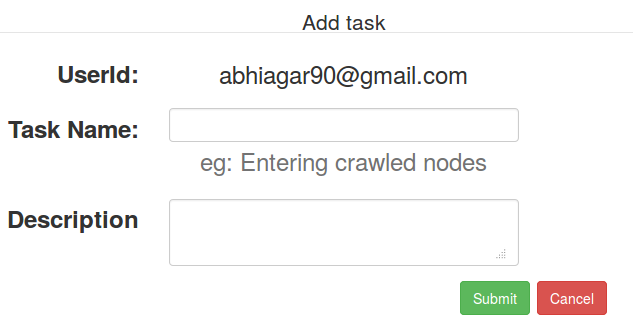
\includegraphics[width=0.6\textwidth]{taskcreate} 
\caption{Creating tasks for a data-gathering group}
\label{fig:taskcreate}
\end{center}
\end{figure}


\begin{figure}[H]
\begin{center}  
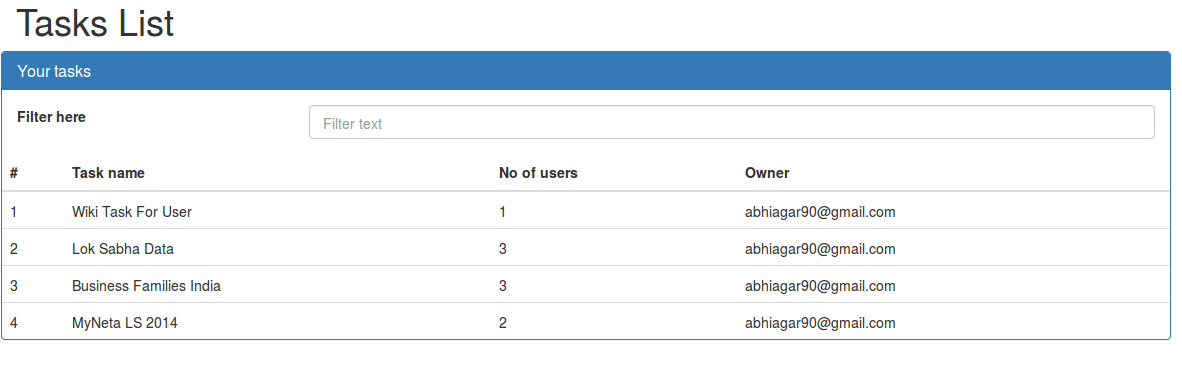
\includegraphics[width=1\textwidth]{tasksall} 
\caption{Information about a task}
\label{fig:tasksall}
\end{center}
\end{figure}


\subsection{User Addition}
By default when a task is created, the owner is automatically added as one the users of the created task.
He can add more users to the task which will allow those users to be able to push data specific to that task \ref{fig:taskadduser}.

\begin{figure}[H]
\begin{center}  
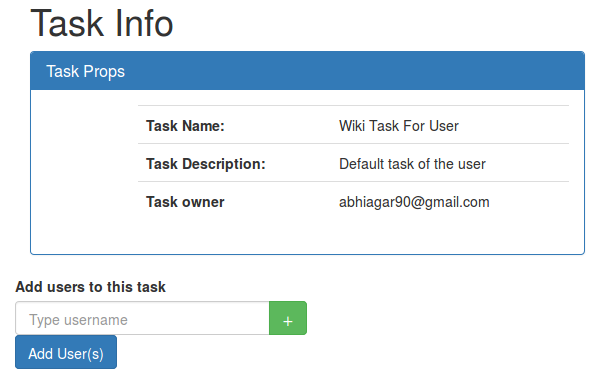
\includegraphics[width=0.7\textwidth]{taskadduser} 
\caption{Adding user to a task}
\label{fig:taskadduser}
\end{center}
\end{figure}


\subsection{Authorization \& POST API}
Every authorized user in the system is given an api-token at the time of sign-up. An api request is authorized if userid and api-token are provided correctly. For pushing data to the system using a valid api-request, json has been employed as the payload. The structure has been described in section [TODO]
To push the JSON to the system, the API request is described in table \ref{tab:postjson}.

\begin{table}[H]
\centering
\caption{Request API: /apis/postgraph/?userid=$\langle userid \rangle$\&token=$\langle userid \rangle$}
\label{tab:postjson}
\begin{tabular}{ll}

\textbf{URL Parameters} & userid, token                              \\

\hline

\textbf{Headers}        & Content-Type : application/json            \\

\hline

\textbf{Payload}        & JSON                                       \\

\hline

\textbf{JSON VARS}      & taskid, userid, token, entities, relations \\
\hline

\textbf{HTTP-METHOD}    & POST      \\
\hline                                

\end{tabular}
\end{table}

\subsection{JSON Response}
If request is authorized and json is as per our convention, then the data is pushed to the crawl data-store. Validations before the push happen as described in the [TODO:section]. The response is almost identical copy of the request json, including the meta-data. All the metdata has been marked with a beginning and an ending underscore \ref{jsonresponse} \\


\label{jsonresponse}
\begin{lstlisting}[language=json,firstnumber=1]
"16": {
      "labels": [
        "person",
        "entity",
        "indian",
        "politician"
      ],
      "properties": {
        "_crawl_en_id_": "en_7_16",
        "_fetchdate_": 1466781745,
        "_nodenumber_": 16,
        "_pushdate_": 1467056465.732715,
        "_pushedby_": "mridul.goel53@gmail.com",
        "_sourceurl_": "https://www.wikipedia.org/",
        "_taskid_": 7,
        "name": "Akhilesh Yadav"
      }
    }
\end{lstlisting}


\section{Resolver and verifier}

\begin{enumerate}

\item \textbf{Use Case:} The use case diagram for verifier is shown in Figure \ref{fig:verifier}


\begin{figure}[H]
\begin{center}  
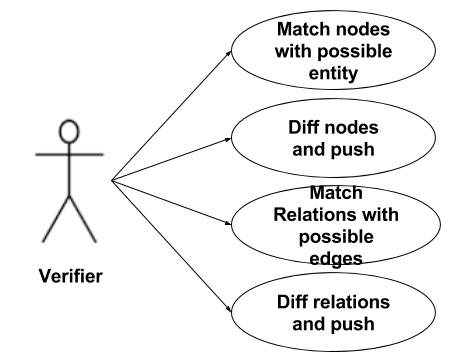
\includegraphics[scale=0.3]{verifier} 
\caption{Use cases for Verifier}
\label{fig:verifier}
\end{center}
\end{figure}
 
\item \textbf{Resolution:} Every node in the crawl data-store has to be resolved to a node (existing or new) in the core data-store, meaning to resolve is to provide it with a uuid. Similarly for relations, a relid is provided. This is achieved when a verifier picks up an object during match \ref{fig:match} from the possible list of objects suggested by the resolver. Diff view \ref{fig:diff} aids the verifier to granularly look at new labels, new properties and conflicting properties (shown with differentiating colors).

\begin{figure}[H]
\begin{center}  
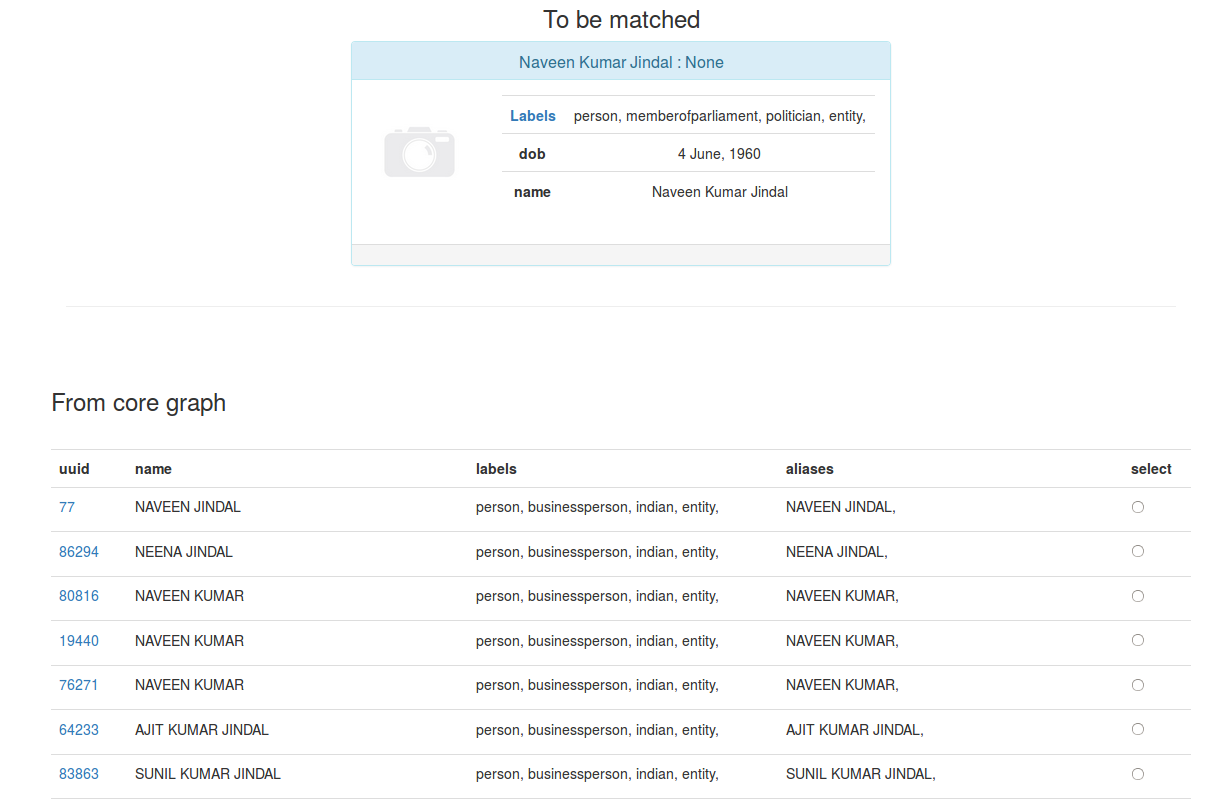
\includegraphics[width=1\textwidth]{match} 
\caption{The match view in verification task}
\label{fig:match}
\end{center}
\end{figure}

\begin{figure}[H]
\begin{center}  
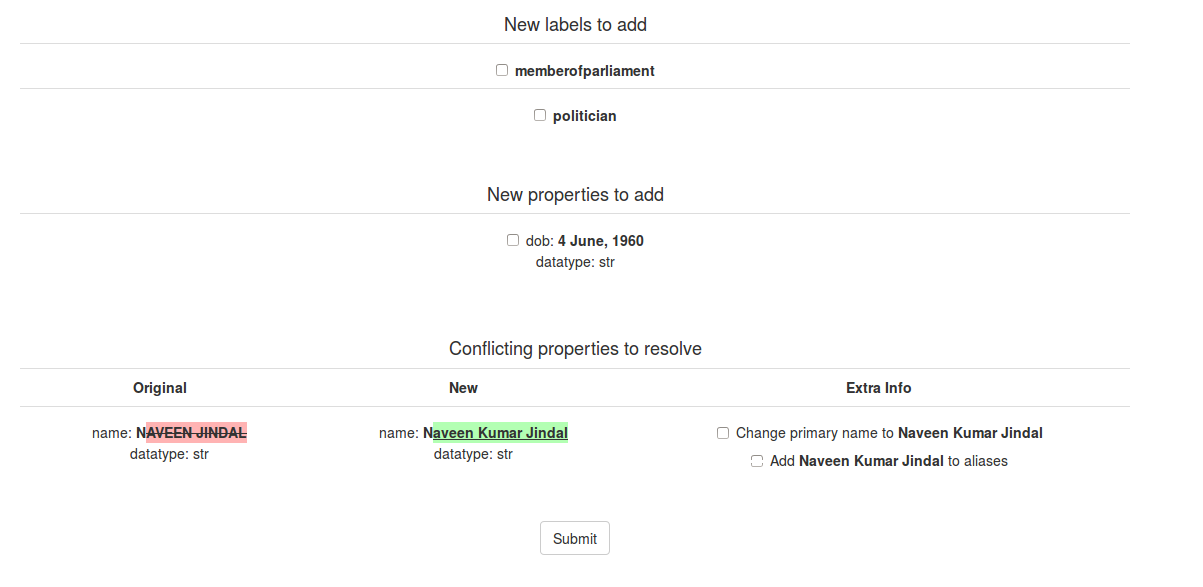
\includegraphics[width=1\textwidth]{diff} 
\caption{The diff view in verification task}
\label{fig:diff}
\end{center}
\end{figure}

\item The key idea is to design views to facilitate the verification task for the verifiers, to help them in focusing on investigating the new information in the least possible time. 

\item \textbf{Selection algorithm:} A selection algorithm picks up the next nodes or relations to resolve. When left with no choice, it picks up the highest degree node, else the node that has the highest number of connected resolved nodes is picked.

\item \textbf{Validations}: Robust validations have been used on match and diff view to ensure that nothing creepy happens at the core data-store. Option to resume an on-going task, clear current session, release all locks have also been provided \ref{fig:session}.

\begin{figure}[H]
\begin{center}  
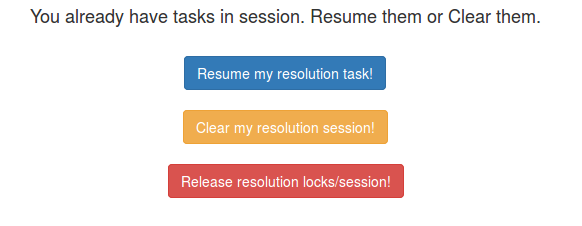
\includegraphics[width=0.7\textwidth]{session} 
\caption{The match view in verification task}
\label{fig:session}
\end{center}
\end{figure}


\item \textbf{Parallelization:} A graph object selected during a verifier's session is locked for some time to let the selection algorithm know of it's status, this way the selection algorithm picks up another potential node.

\item \textbf{Jaro:} Provision for running jaro on fetched entities from Apache Solr has been provided in the match view. In practice, phonetic has been seen to be do very well for names we have encountered. We have kept this feature extensible in the sense if some other algorithms need to be tested for the task.

\item \textbf{Multi valued-properties:} Extensive care has been taken to incorporate multi-valued property for nodes and relationships. During the diff task, a merge request on the property can result in converting the original value of the property to a multi-valued one. 

\end{enumerate}




% \subsection{Guideline for the verification task}

% a mini-guide to manual verification -- reema sarkar -- [an image]
% very imp as only write happens through verifier
% shortest path
% expand on nodes in neo4j yuvraj singh a falase case can describe
% examples of connection --- between sons etc. 
% screenshots verifier \\
 

\section{Authorized User and Wiki}

\begin{enumerate}

\item \textbf{Use Case:} Use case diagram for authorized users is shown in Figure \ref{fig:registereduser}.

\begin{figure}[H]
\begin{center}  
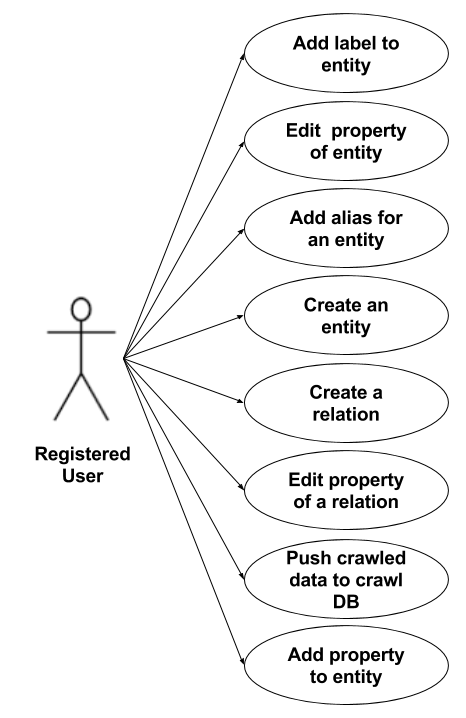
\includegraphics[scale=0.4]{registereduser} 
\caption{Use cases for registered users.}
\label{fig:registereduser}
\end{center}
\end{figure}

\item \textbf{Wiki:} Authorized users can access the wiki to edit entities and relationships in the core data-store. All these edits are first sent to the crawl data-store in the same fashion as any json from a data-gatherer is handled. This way all changes in the system occur through the verification process to have the core data-store free of any noise or redundancy. 


\item \textbf{Wiki features:} Wiki can be accessed to add a new node, add a  new relation \ref{fig:addrel},  edit an existing node  - add a new label \ref{fig:addlabel}, edit an existing relation. A user can add as many properties to the entity/relationship as possible \ref{fig:oldprops}. Certain properties that can be potential candidates for addition are also suggested in the edit view \ref{fig:oldprops}. 

\begin{figure}[H]
\begin{center}  
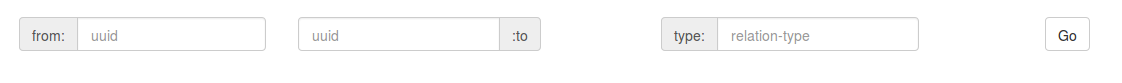
\includegraphics[width=1\textwidth]{addrel} 
\caption{Add relation between two entities}
\label{fig:addrel}
\end{center}
\end{figure}


\begin{figure}[H]
\begin{center}  
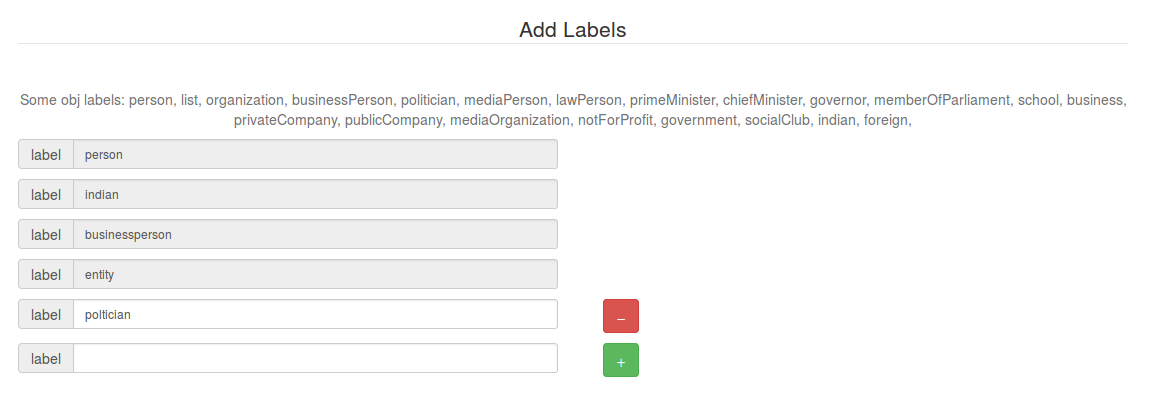
\includegraphics[width=1\textwidth]{addlabel} 
\caption{Add new labels to a node}
\label{fig:addlabel}
\end{center}
\end{figure}

\begin{figure}[H]
\begin{center}  
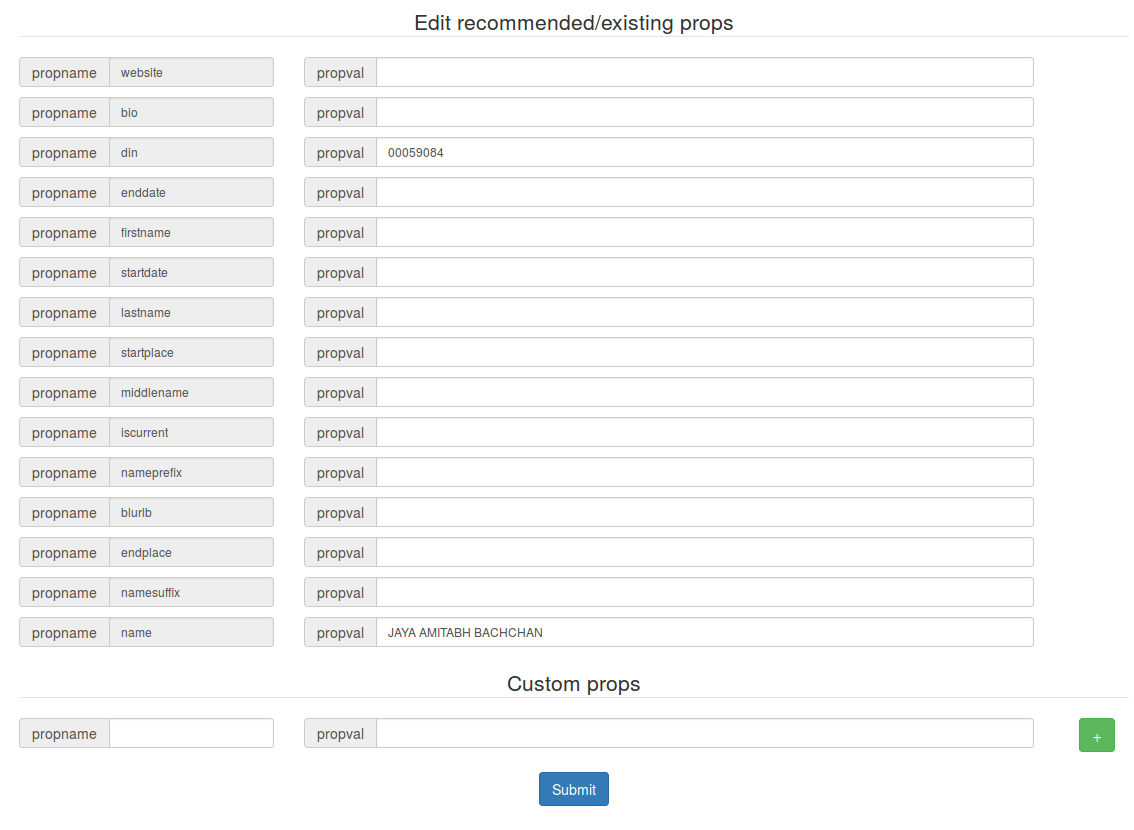
\includegraphics[width=1\textwidth]{oldprops} 
\caption{Edit existing properties/Add recommended properties}
\label{fig:oldprops}
\end{center}
\end{figure}



\end{enumerate}


\section{Provenance}

\begin{enumerate}

\item \textbf{Accountability:} We felt the need to maintain every granular detail about any change in the core data store. Thus, a label addition, a property change, a property addition, all need to be accounted for - who pushed the change, when was it pushed, when was the data collected by the data-gatherer, who verified the change, the source-url for the new information, etc.

\item \textbf{Meta-DB:} All this meta-data is stored on a dedicated MySQL back-end that is updated as soon as a new updation is approved by the verifier. 

\item \textbf{History:} A history feature on the web application for each entity and for each relation helps an end user to see our provenance meta-data. The same is better viewed in Figure \ref{fig:prov1} and Figure \ref{fig:prov2}.

\begin{figure}[H]
\begin{center}  
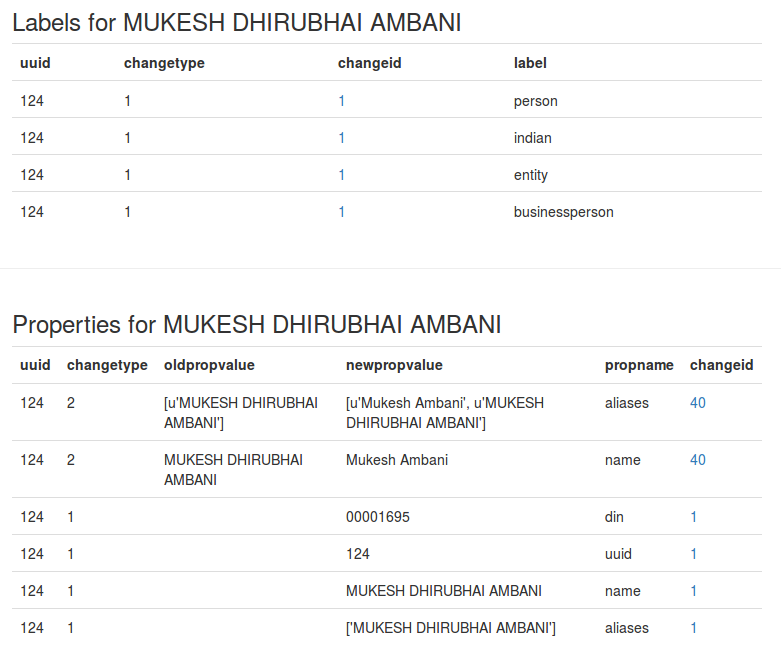
\includegraphics[scale=0.4]{prov1} 
\caption{Every change is attributed to a change ID}
\label{fig:prov1}
\end{center}
\end{figure}


\begin{figure}[H]
\begin{center}  
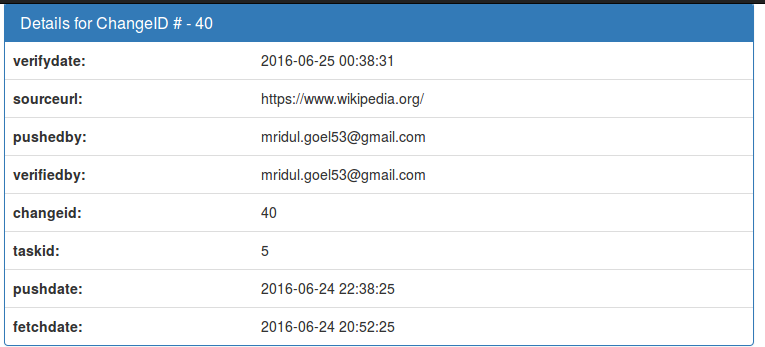
\includegraphics[scale=0.5]{prov2} 
\caption{Every change has an associated meta-data}
\label{fig:prov2}
\end{center}
\end{figure}


\end{enumerate}





\section{End user}

\begin{enumerate}

\item \textbf{Use Case:} Use case diagram for not logged in end users is shown in Figure \ref{fig:enduser}.

\begin{figure}[H]
\begin{center}  
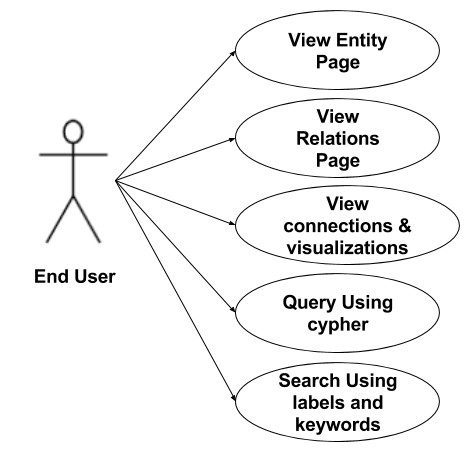
\includegraphics[scale=0.3]{enduser} 
\caption{Use cases for End User}
\label{fig:enduser}
\end{center}
\end{figure}




\item \textbf{Search:} End user can search for entities in our core data store. The search is powered by Apache Solr and uses double metaphone. The search can be filtered on labels and keywords. An actual search query is shown in Figure \ref{fig:endsearch} 

\begin{figure}[H]
\begin{center}  
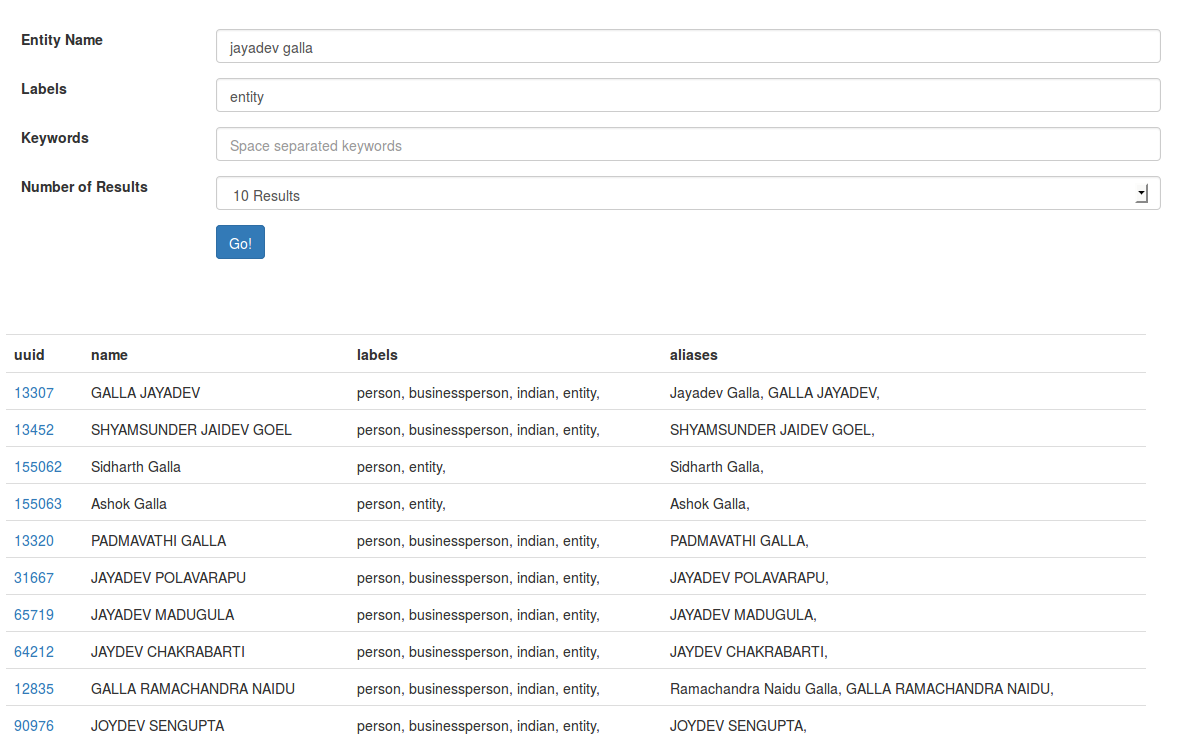
\includegraphics[scale=0.3]{endsearch} 
\caption{Search Page results}
\label{fig:endsearch}
\end{center}
\end{figure}


\item \textbf{View entity profiles and connections:} User can browse to profile pages of entities in our core data-store. The profile shows information about the particular entity and also displays first level relations for the same. An actual profile from the core data-store and connections for the same entity are shown in Figure \ref{fig:endprofile} and \ref{fig:endconnections} respectively.


\begin{figure}[H]
\begin{center}  
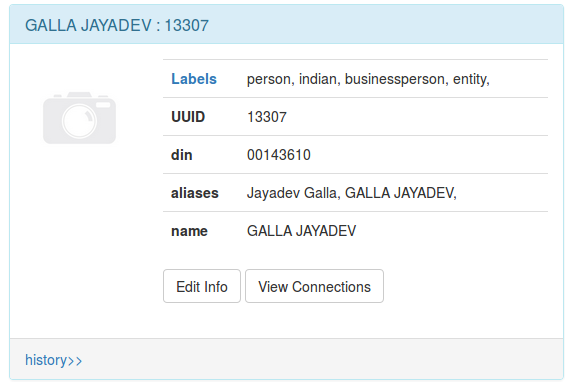
\includegraphics[width=0.6\textwidth]{endprofile} 
\caption{Entity profile from core data-store}
\label{fig:endprofile}
\end{center}
\end{figure}



\begin{figure}[H]
\begin{center}  
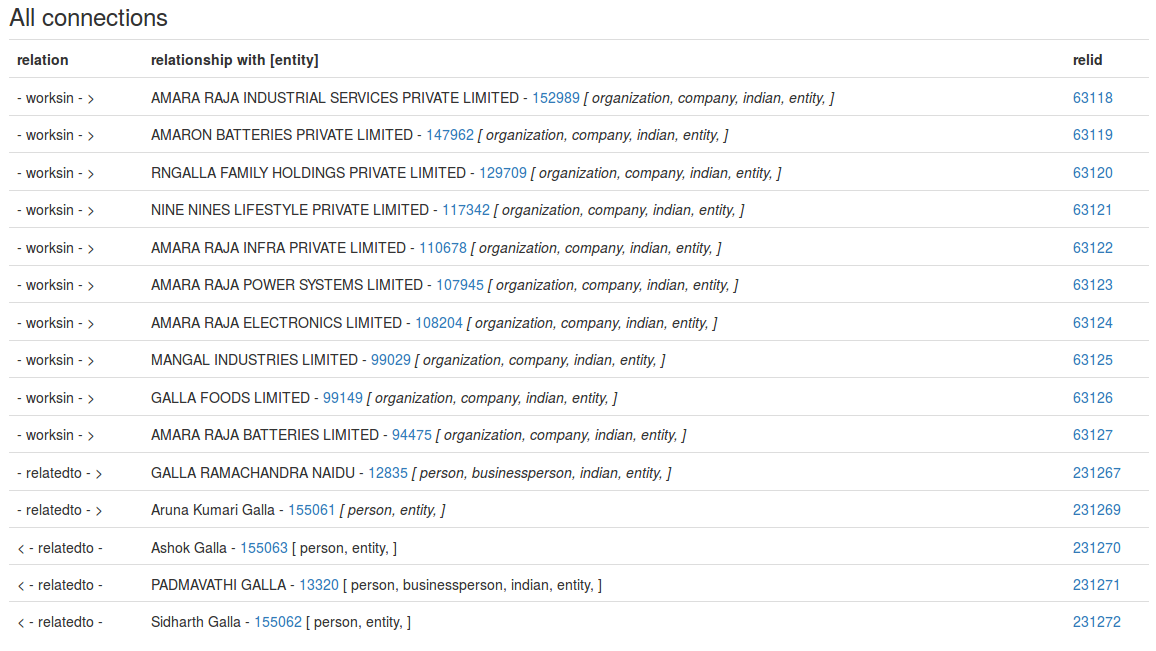
\includegraphics[scale=0.3]{endconnections} 
\caption{Entity connections from core data-store}
\label{fig:endconnections}
\end{center}
\end{figure}


\item \textbf{Visualizations for the end user:} The end user can generate visualizations for a cypher query. The cypher query is first validated for safety and load, and then executed. Result of an actual cypher query is shown in Figure \ref{fig:endviz}.

\begin{figure}[H]
\begin{center}  
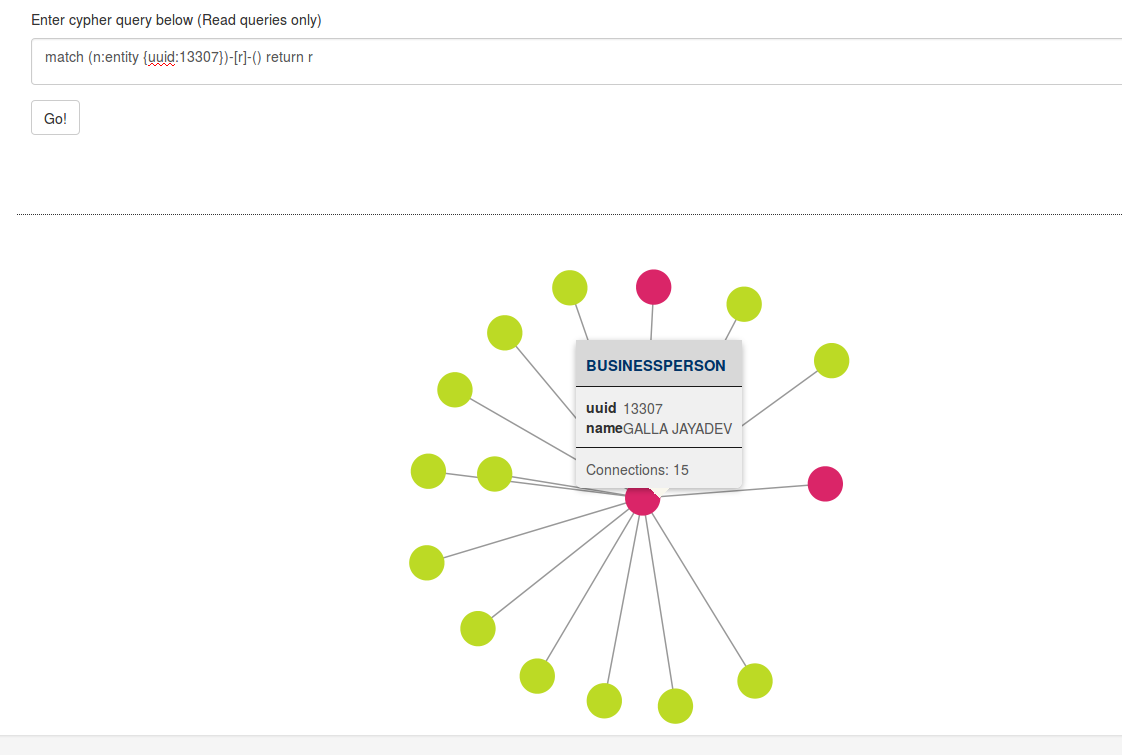
\includegraphics[width=1\textwidth]{endviz} 
\caption{End user generates visualization}
\label{fig:endviz}
\end{center}
\end{figure}


\end{enumerate}

% database model er diagrm sanphot meta db - index table also include?? [left] \\


\section{Admin}

\begin{enumerate}
    \item \textbf{Use Case:} Use case diagram for not logged in end users is shown in Figure \ref{fig:admin}.

    \begin{figure}[H]
    \begin{center}  
    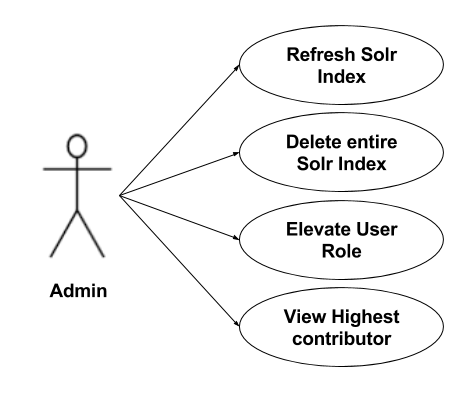
\includegraphics[scale=0.3]{admin} 
    \caption{Use cases for Admin}
    \label{fig:admin}
    \end{center}
    \end{figure}
    

     \item \textbf{Solr Indexes:} Admin can delete all the Solr indexes, and can also refresh them for maintenance purposes.

     \item \textbf{Change user roles:} Admin can change roles of existing authorized users, so a user role in the system is always controlled by the admins.


     \item \textbf{View contributions:} Admin on a broader level needs to look over the verification/moderation process in the system. Towards that effect, an admin can view all the statistics about verifiers and data-gatherers present in the system.

     \item \textbf{Bots:} Not all the tasks can be done by humans alone, and thus we have introduced the concept of bots in the system. All these bots wake up at regular intervals and execute any background jobs scheduled for them. All these bots thus need to have admin roles for this purpose. We have a \emph{Location resolver bot} that periodically checks if any entity has an address field and is not connected to any city. It then automatically parses the address and introduces a relation from that entity to that city. We also have a \emph{Dangling locks release} bot that releases any dangling locks in the crawl data store after a specified interval.   

\end{enumerate}

\chapter{Results and Visualizations}

When we started out the initial core data set contained mostly director sharing data. The process of data collection for this dataset is described in data collection section [cite todo section]. Interesting insights come about when we dig inside this dataset and try to find how a big entity is connected to another big entity. \\

Interesting results come about when we merged this dataset with family trees and political data that we obtained. Though list is a bit long, we have tried to document only the best examples here. \\

We have just been able to touch three realms here: corporate, political, entertainment.
Also, we have tried to see family trees to validate nepotist practices in politics and businesses. \\

The idea through these visualizations is to show that the power houses interact and mingle among themselves. \\

% 1. sons, daughters, wives, parents, in-lawas share board of director positions
% 2. marraiges in nig power houses among big power houses -- link established explicilty
% 3. business tycoons come baout together to become board of directors
% 4. fmaily trees for corporates large
% 5. politcians and their families linked to croporate realm
% 6. cricketers and their corporate links

\section{Influence Network}

Here we describe the case of politician and business tycoon Naveen Jindal. He is directly on the board of 8 companies. Through director sharing, in 2 hops, he spans 144 companies, in 3 hops the span network is greater than 1800 companies.Interestingly in 4 hops, his influence network reaches more than 13000 companies out of the 60000 companies network we have in our DB!  Naveen Jindal is connected to (within 3 hops): Ashok Leyland, Ambuja cements, Reliance Power, Indiabull, ONGC, JP Associates, Idea, Essar, IDFC, Tata Motors, Shriram, Bharti, Max Life, IDBI, Mahindra, BPCL, Network 18, BHEL, Lanco, Maruti Suzuki, ICICI Bank, Infosys, Adani, ITC, Tech Mahindra, Wipro, HDFC, Hinduja, DLF, Indraprastha Gas, Dabur India, Jet Aiarways, JK Lakshmi Cement, ad nauseum. It is as if every big company is connected to the other: really the Power Elites! And to top that, he was an MP for ten years.


\begin{figure}[H]
\begin{center}  
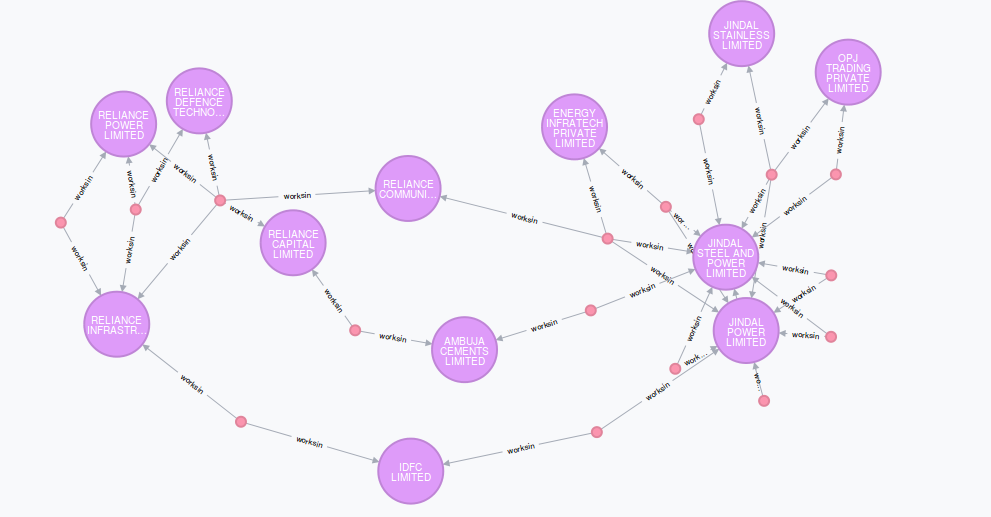
\includegraphics[width=1\textwidth]{nj1} 
\caption{Naveen Jindal's connections with Reliance}
\label{fig:nj1}
\end{center}
\end{figure}

\begin{figure}[H]
\begin{center}  
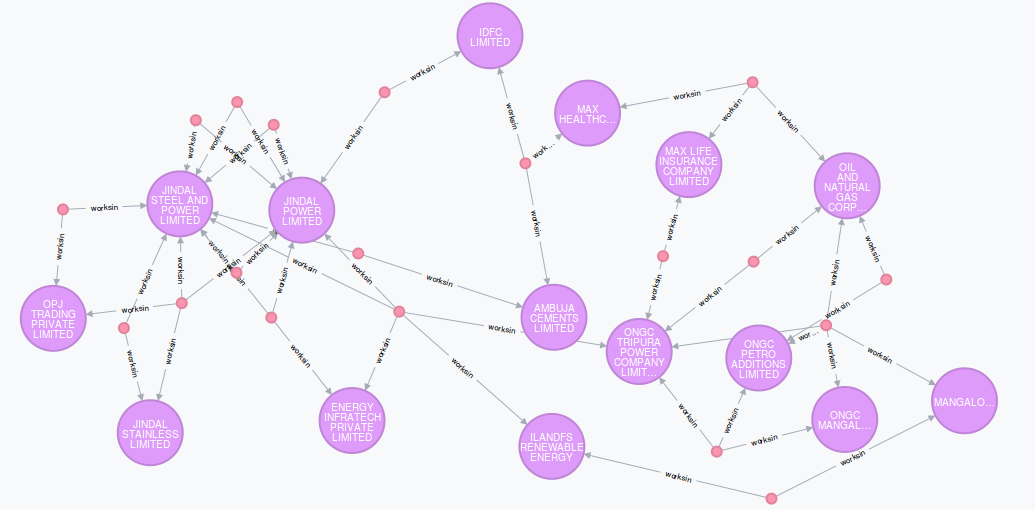
\includegraphics[width=1\textwidth]{nj2} 
\caption{Naveen Jindal's connections with Ambuja Cement and ONGC}
\label{fig:nj2}
\end{center}
\end{figure}


\section{Intersting directors}

\subsection{Not just Mahindra}
\begin{figure}[H]
\begin{center}  
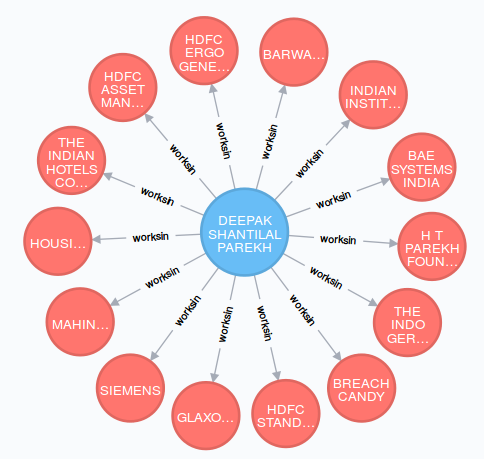
\includegraphics[width=0.4\textwidth]{parekh} 
\caption{Deepak parekh and his first-level directors}
\label{fig:parekh}
\end{center}
\end{figure}


\subsection{The Lavasa Connection}
\begin{figure}[H]
\begin{center}  
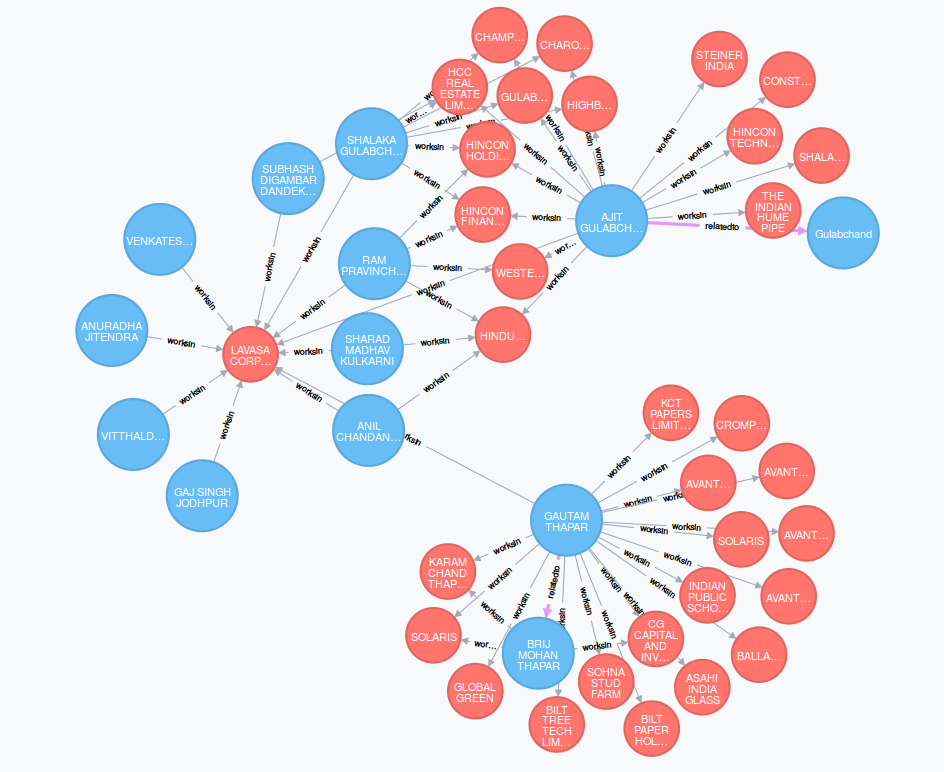
\includegraphics[width=1\textwidth]{lavasa} 
\caption{Gulabchands and Thapars}
\label{fig:lavasa}
\end{center}
\end{figure}


\section{Media Houses}

\subsection{Birlas, HT and Ambanis}

\begin{figure}[H]
\begin{center}  
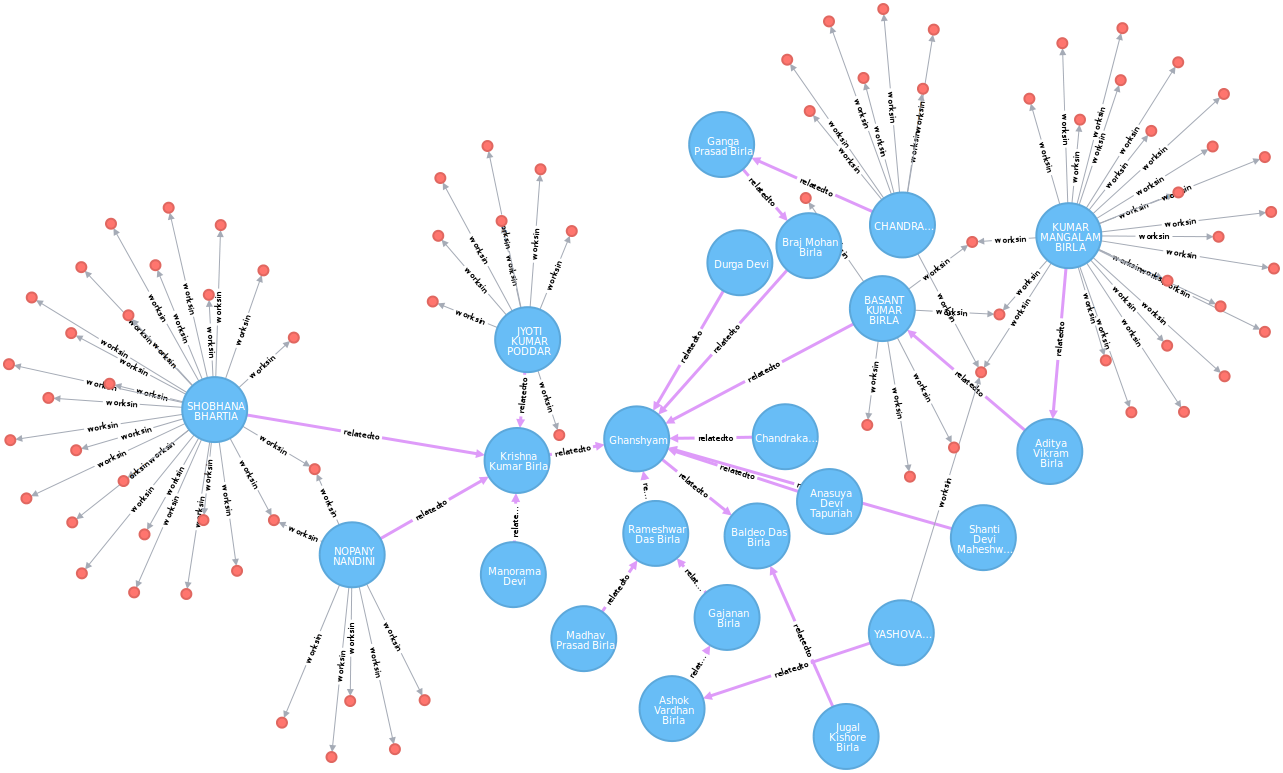
\includegraphics[width=1\textwidth]{ht} 
\caption{Shobhana Bhartia, Hindustan Times owner, ex-Rajya Sabha MP}
\label{fig:ht}
\end{center}
\end{figure}

\subsection{The Sarkars}

\begin{figure}[H]
\begin{center}  
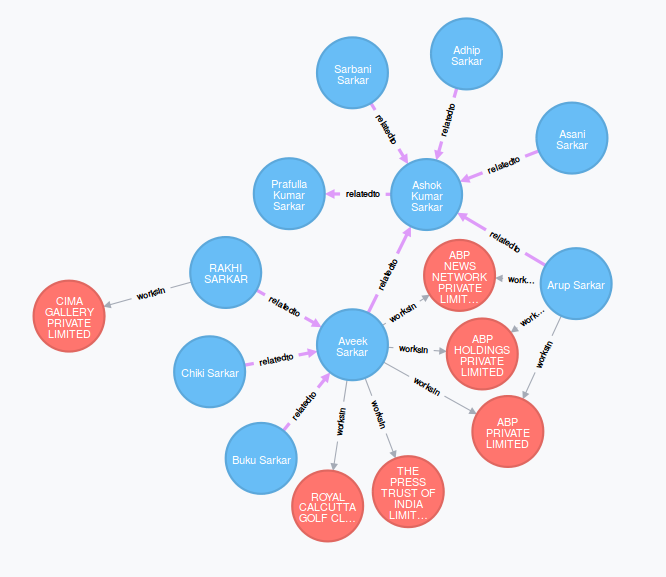
\includegraphics[width=1\textwidth]{sarkar} 
\caption{Aveek Sarkar of the Telegraph and ABP group}
\label{fig:sarkar}
\end{center}
\end{figure}


\section{Family trees}

\subsection{Ambani's}

\begin{figure}[H]
\begin{center}  
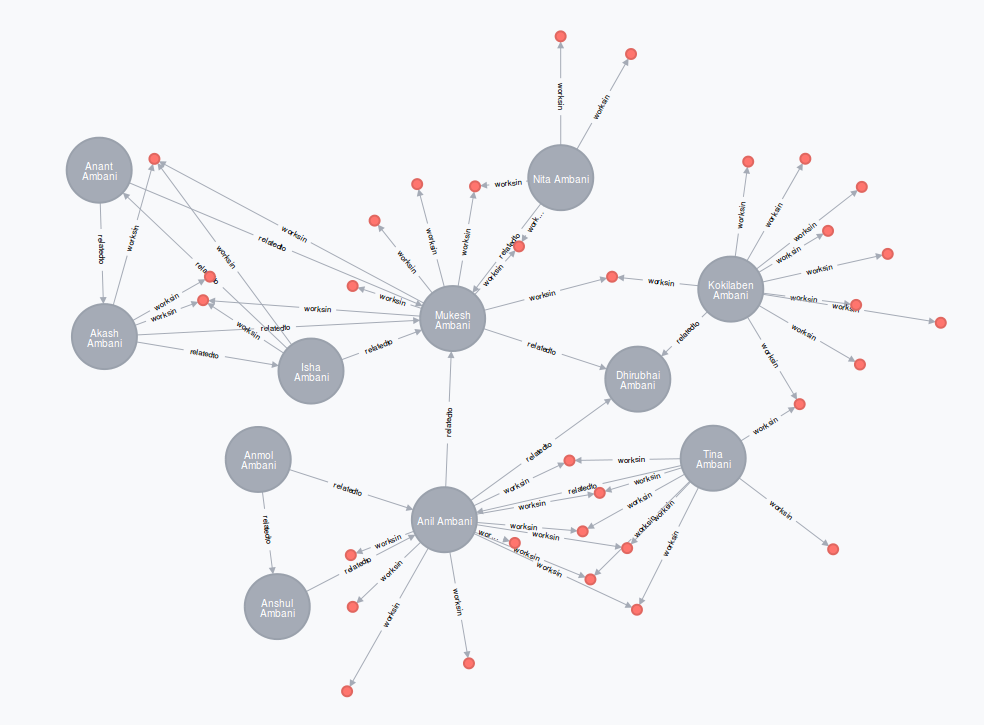
\includegraphics[width=1\textwidth]{ambani} 
\caption{Reliance: It's all in the family}
\label{fig:ambani}
\end{center}
\end{figure}


\subsection{The better halves}

\begin{figure}[H]
\begin{center}  
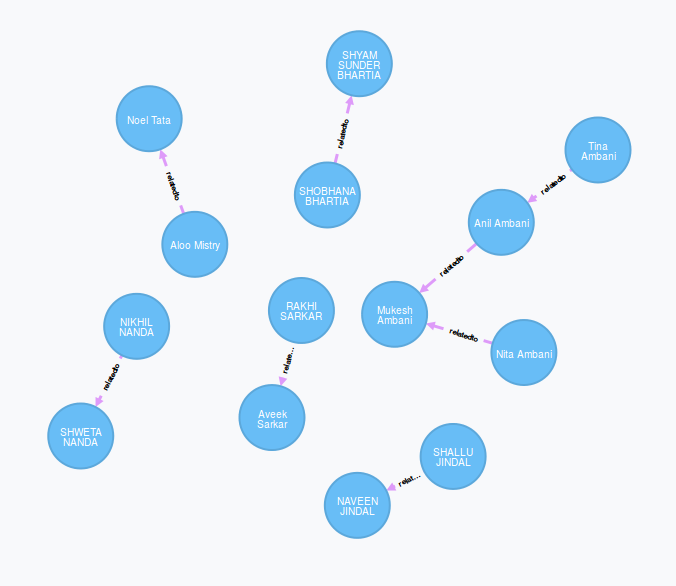
\includegraphics[width=0.8\textwidth]{spouses} 
\caption{Businesswomen and also spouses}
\label{fig:spouses}
\end{center}
\end{figure}


\subsection{Yadavs from UP and Bihar}

\begin{figure}[H]
\begin{center}  
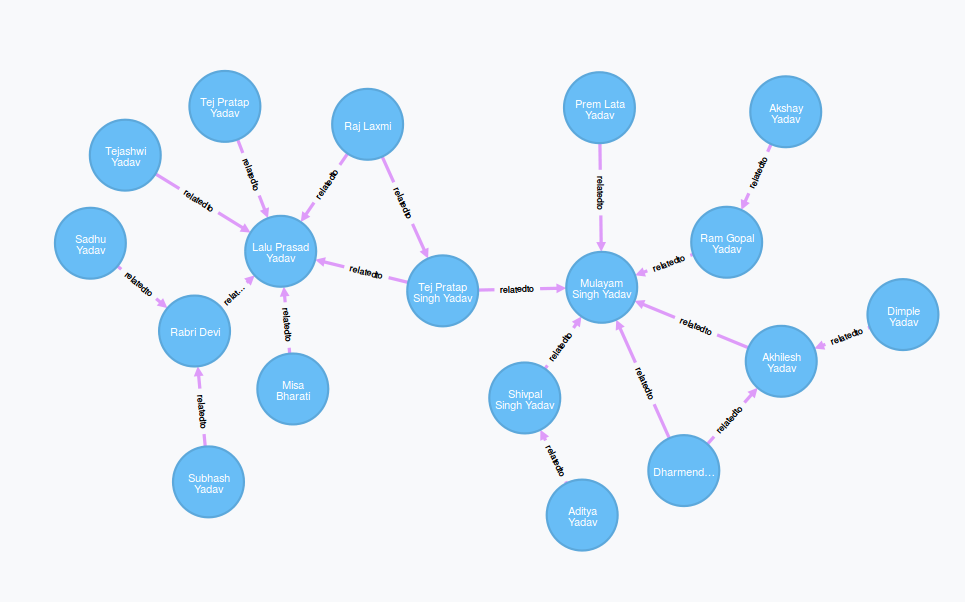
\includegraphics[width=0.8\textwidth]{yadavs} 
\caption{Connection between Lalu Prasad Yadav and Mulayam Singh Yadav}
\label{fig:yadavs}
\end{center}
\end{figure}


\section{Runaways or corporate hulks}

\subsection{Modis of Modinagar}

\begin{figure}[H]
\begin{center}  
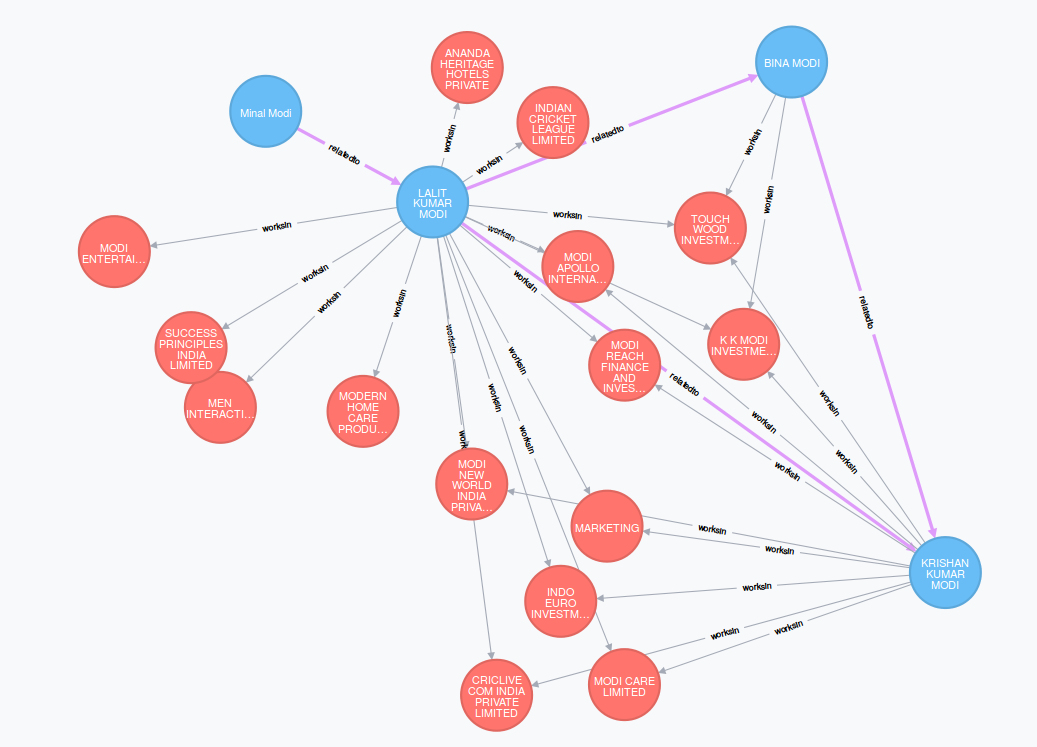
\includegraphics[width=1\textwidth]{modi} 
\caption{Lalit Modi of Modi dynasty}
\label{fig:modi}
\end{center}
\end{figure}


\subsection{Mallyas}

\begin{figure}[H]
\begin{center}  
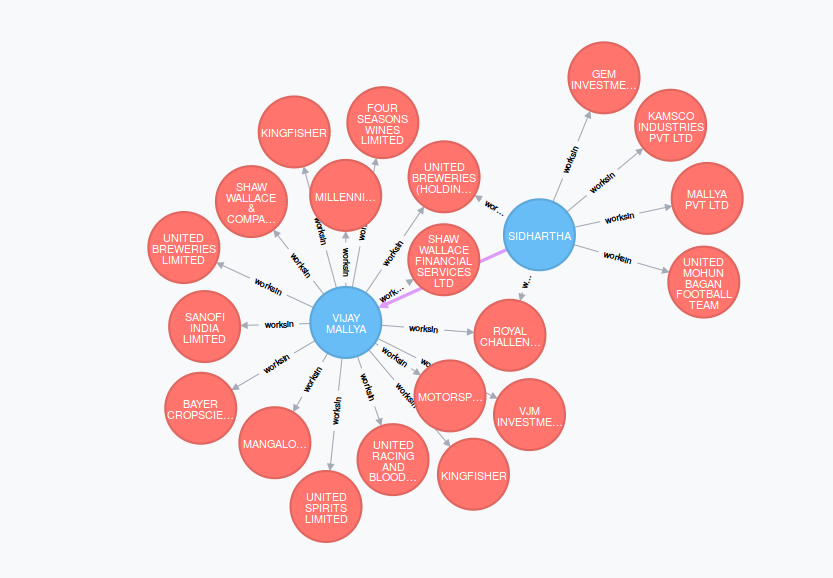
\includegraphics[width=1\textwidth]{mallya} 
\caption{Vijay mallya's empire}
\label{fig:mallya}
\end{center}
\end{figure}

\section{Arts, sports and commerce}

\subsection{Bacchchans, Nandas, \& Kapoors}

\begin{figure}[H]
\begin{center}  
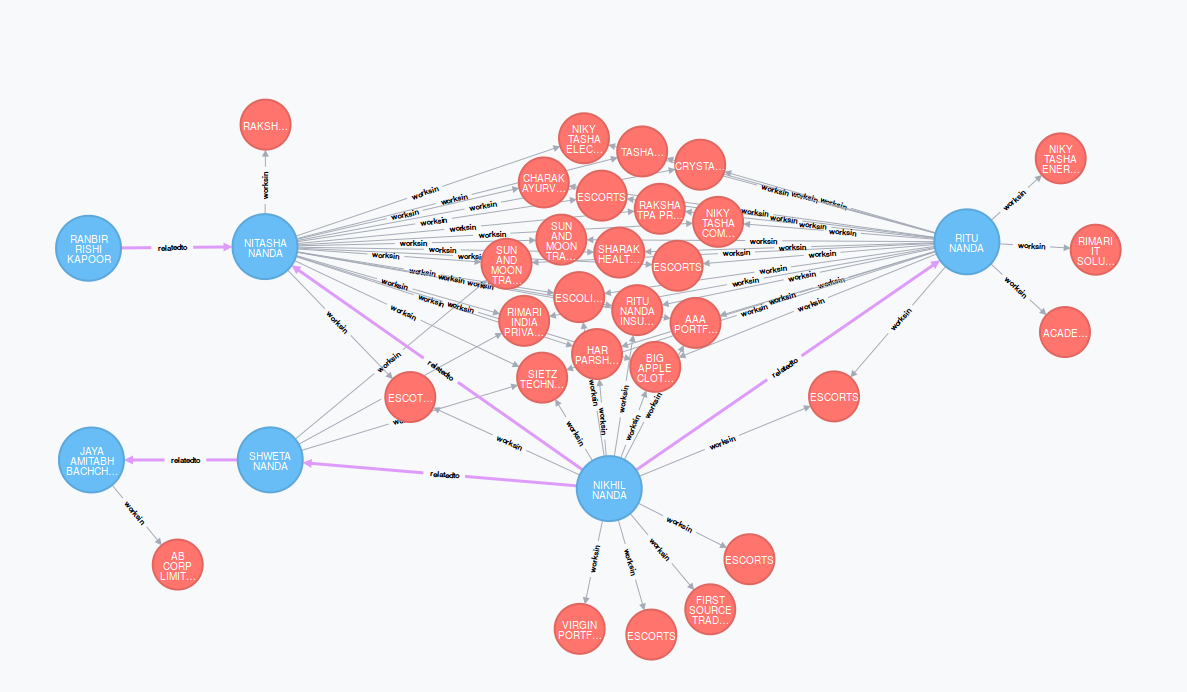
\includegraphics[width=1\textwidth]{nanda} 
\caption{One of the best examples of big houses marrying richer/bigger houses}
\label{fig:nanda}
\end{center}
\end{figure}

\subsection{King's XI Punjab and the boyfriend connection}

\begin{figure}[H]
\begin{center}  
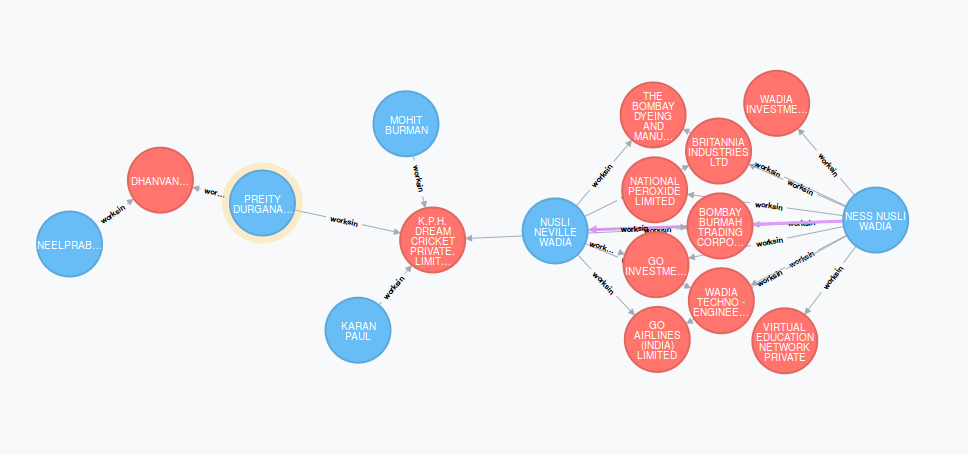
\includegraphics[width=1\textwidth]{wadia} 
\caption{Preity Zinta, holding a directorship in KXP, with the then-boyfriend Ness Wadia}
\label{fig:wadia}
\end{center}
\end{figure}

\subsection{Dada's family and business}

\begin{figure}[H]
\begin{center}  
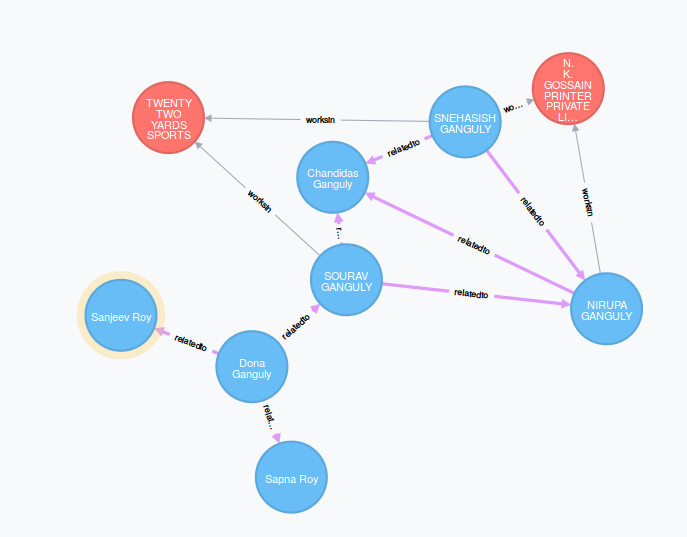
\includegraphics[width=1\textwidth]{ganguly} 
\caption{Sourav Ganguly and his company; his father is one the richest men in Kolkata}
\label{fig:ganguly}
\end{center}
\end{figure}



\section{Politics and Corporate}

There are numerous well known examples like Naveen Jindal and Jaydev Galla that recur time and gain in news. Here we mention some more.

\subsection{Gandhis and Vadra}

\begin{figure}[H]
\begin{center}  
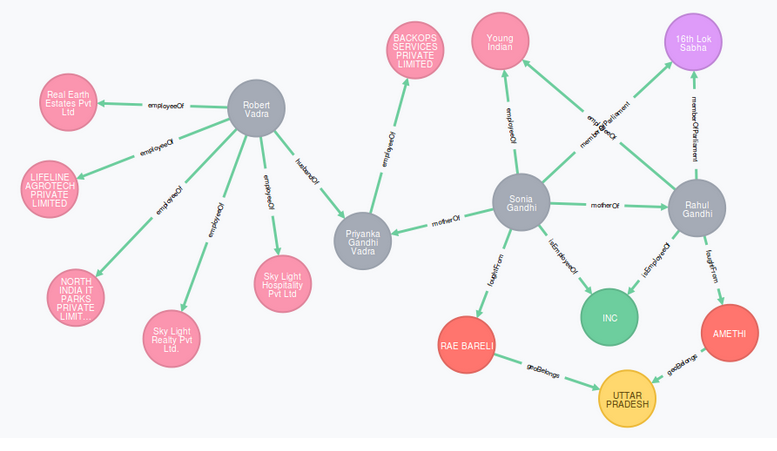
\includegraphics[width=1\textwidth]{gandhi} 
\caption{Gandhis and Son-in-law Vadra}
\label{fig:gandhi}
\end{center}
\end{figure}

\subsection{Jayant Sinha and his business-cum-political family}

\begin{figure}[H]
\begin{center}  
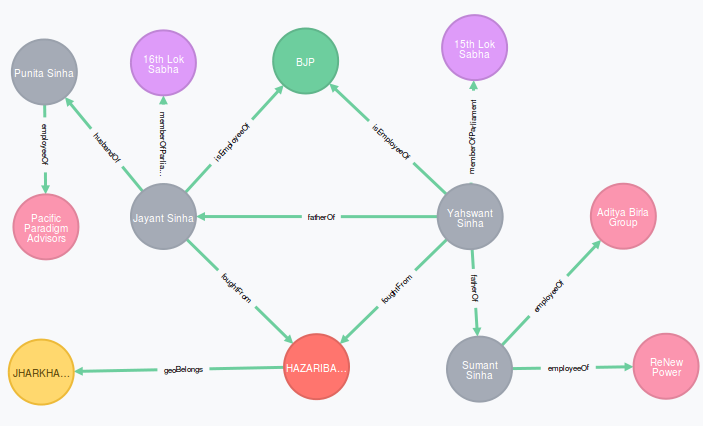
\includegraphics[width=1\textwidth]{sinha} 
\caption{Jayant Sinha and Family}
\label{fig:sinha}
\end{center}
\end{figure}

\subsection{Kamal Nath and Moserbaer}

\begin{figure}[H]
\begin{center}  
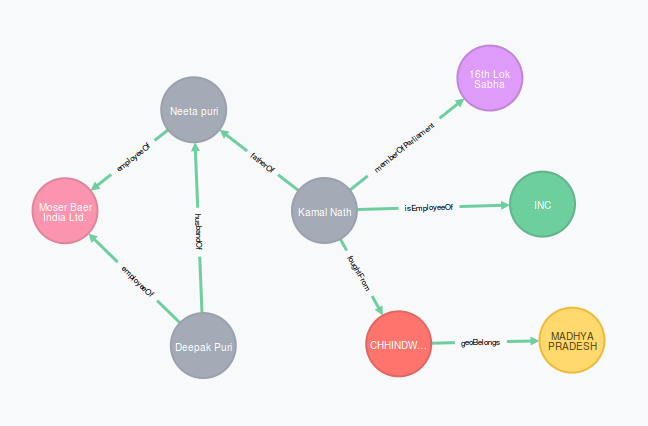
\includegraphics[width=1\textwidth]{nath} 
\caption{Kamal Nath and family}
\label{fig:nath}
\end{center}
\end{figure}

\bibliographystyle{plain}
\bibliography{biblio}

%\appendix
%\chapter{CHAPTER NAME}

\section{SECTION NAME}
\lipsum[1]

\section{SECTION NAME}
\lipsum[2]

\end{document}
